
\chapter{Share: HapTurk}
\label{ch:hapturk}


\begin{figure}[h] %  figure placement: here, top, bottom, or page
   \centering
   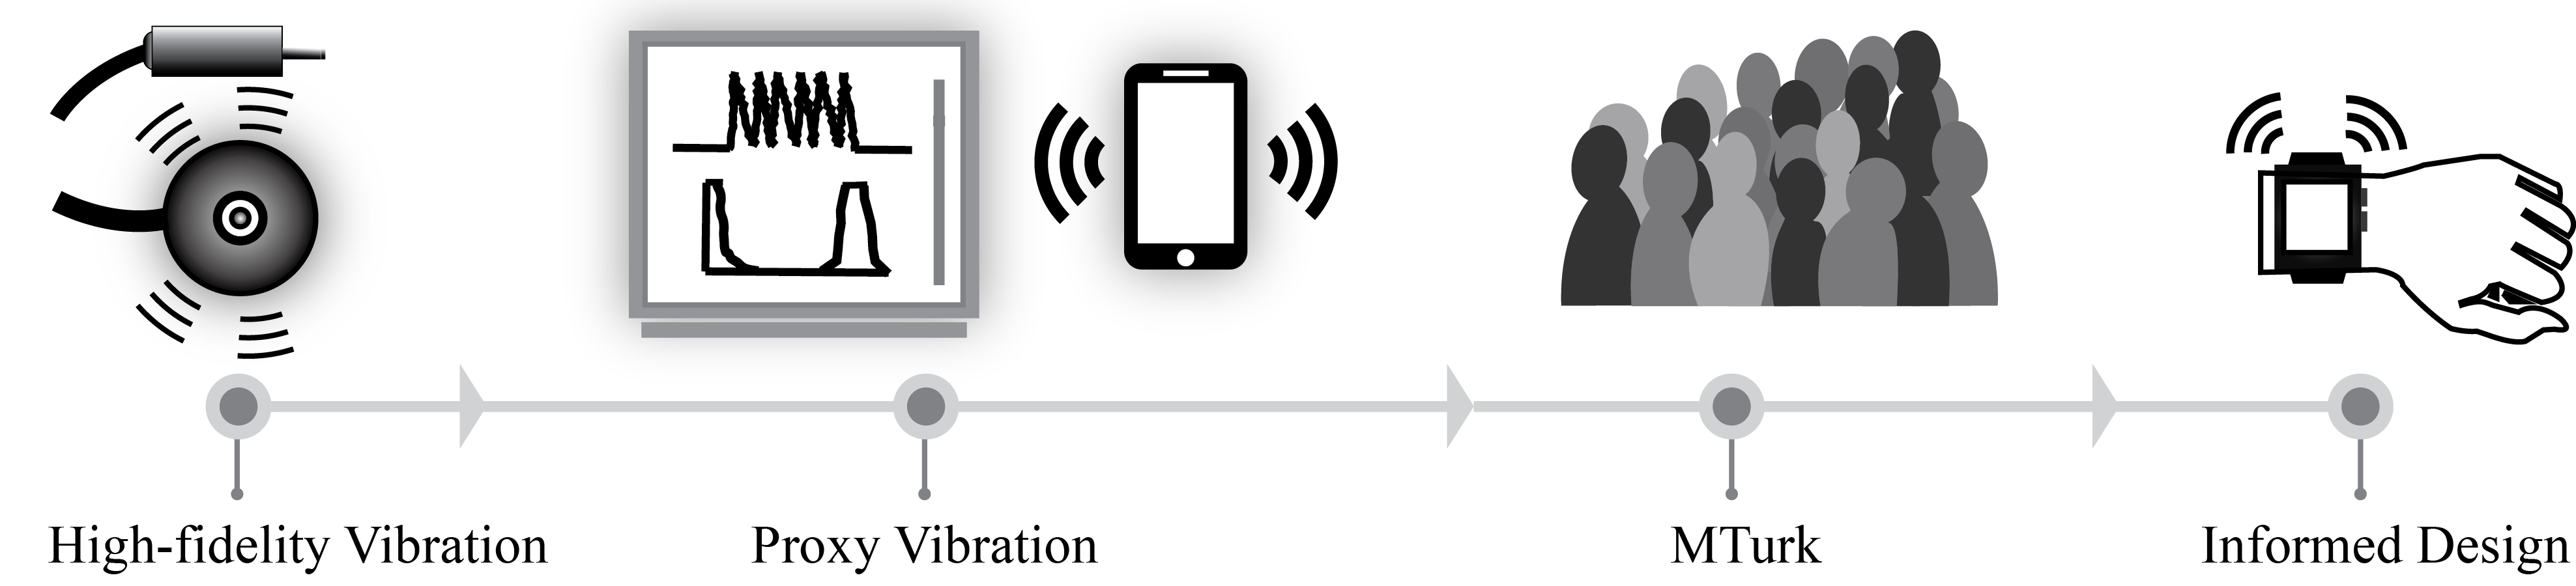
\includegraphics[width=\textwidth]{ConceptSketch-03} 
   \caption{In HapTurk, we access large-scale feedback on informational effectiveness of high-fidelity vibrations after translating them into proxies of various modalities, rendering important characteristics in a crowdsource-friendly way.}
   \label{fig:hapturk:conceptsketch}
\end{figure}


\noindent
\inlineHeading{Preface} 
While Chapters \ref{ch:hapticinstrument}-\ref{ch:macaron} describe iterative development of vibrotactile tools, \osE{with} HapTurk\footnote{\fullCitation{Schneider2016hapturk}} \osE{we} stud\osE{y} a vibrotactile technique. % to support large scale feedback high-fidelity VT effects.
Here, we look into \emph{browse}'s \osE{inverse}: \emph{share}, disseminating or storing a design concept for others' use.
\osE{We focus on one aspect of \emph{sharing}: disseminating designs over the internet. In this case, the goal is to collect large-scale feedback.}
%\osE{This follows} up on our goal of \osE{supporting} collaboration in \autoref{ch:hapticinstrument}, where we found utility in \osE{\emph{sharing} designs informally for feedback.} 
%informal, collocated user feedback. %, but were unable to reach conclusions about haptic language due to small sample size.
%We specifically study \emph{sharing} in the context of collecting feedback.
In other design domains, crowdsourcing platforms like Amazon's MTurk can deploy user studies \osE{and rapidly collect} large samples.
%    The  problem with crowdsourcing tactile feedback is that the ``crowd''  can't feel the stimuli.
   % Even when consumer devices have tactors,  output quality and intensity is unpredictable and uncontrollable.
%    Sending each user a device is impractical
%   What we need are crowd-friendly proxies for test stimuli.
However, high-fidelity haptic sensations require specialized \osE{hardware, which most crowdsourced participants will not be able to access}.
\osE{We instead send} more easily-shared stimuli: proxies, \osE{like visualizations and low-fidelity phone vibrations.} %which are sent to the crowd instead of the source stimuli.
\osE{We found these proxies can convey some affective characteristics for some source stimuli, and identified several directions for developing better proxies.}
%Though we use proxies to collect crowdsourced feedback, this technique be used for other \emph{sharing} purposes, \eg, online media broadcasting.
%In this chapter, we design and evaluate the potential of two proxy methods for high-fidelity vibrations: visualizations and low-fidelity phone vibrations.



%There is ample need for huge-sample haptic evaluation. User experience of transmitted sensations must be robust to receiving device diversity.
%Techniques to broadcast haptic effects to video \cite{Modhrain2001,Kim2009}, e.g., with YouTube \cite{AbdurRahman2010} or MPEG7 \cite{Eid2006,Ferre2008} now require known high-fidelity devices  because of remote device uncertainty;  
%the same applies to social protocols developed for remote use of high-quality vibrations, e.g. in collaborative turn taking \cite{Chan2008}. 
%Elsewhere, studies of VT use in consumer devices need larger samples: e.g., 
%perceivability~\cite{Kaaresoja2005}, encoding of caller parameters \cite{Brown2006mobilealerts}, including caller
%emotion and physical presence collected from pressure on another handset~\cite{Hoggan2012}, and usability of expressive, customizable VT icons in social messaging~\cite{Israr2015}.
%To our knowledge, this is the first attempt to run a haptic study on a crowdsource site and characterize its feasibility and challenges for haptics. 
%


\section{Abstract}
% New actuators for handhelds and wearable devices are making 
    Vibrotactile (VT) display is becoming a standard component of informative user experience, where notifications and feedback must convey information eyes-free.
    However, effective design is hindered by 
    incomplete understanding of relevant perceptual qualities.
    %, together with 
    %the need for user feedback to be accessed in-situ. 
    To access evaluation streamlining now common in visual design, we introduce \emph{proxy modalities} as a way to crowdsource VT sensations by reliably communicating high-level features through a crowd-accessible channel. 
    We investigate two proxy modalities to represent a high-fidelity tactor: a new VT visualization, % technique 
    and low-fidelity vibratory translations playable on commodity smartphones. % such as those in modern wearables.
    We translated 10 high-fidelity vibrations into both modalities, 
    % In two user studies, we evaluate proxy ability to convey affective features and  their consistency when deployed over Mechanical Turk.
    and in two user studies found that both proxy modalities can communicate affective features, and are consistent when deployed remotely over Mechanical Turk. 
    We analyze fit of features to modalities, and suggest  future improvements.
    
    
    
    \section{Introduction}
    
    In modern handheld and wearable devices, vibrotactile (VT) feedback can provide unintrusive, potentially meaningful cues through wearables in on-the-go contexts~\cite{Brunet2013a}.
    With % trend-setting 
    consumer wearables like Pebble and the Apple Watch featuring high-fidelity actuators, VT feedback is becoming standard  in more user tools.
    Today, VT designers seek to provide sensations with various perceptual and emotional connotations to support the growing use cases for VT feedback (everyday apps, games, etc.).
    Although low-level design guidelines exist and are helpful for addressing perceptual requirements \cite{MacLean2003,InwookHwang2013,Ternes2008,Brewster2004,Brown2006a},  higher-level concerns and design approaches to increase their usability and information capacity (e.g., a user's desired affective response, or affective or metaphorical interpretation) have only recently received study and are far from solved \cite{Obrist2013,Arab2015,Seifi2014,Israr2014,Jansson-Boyd2011,Okamoto2013}.
    Tactile design thus relies heavily on iteration and user feedback \cite{Schneider2014}. Despite its importance \cite{Seifi2014,Seifi2015}, collecting user feedback on perceptual and emotional (i.e., affective) properties  of tactile sensations in small-scale lab studies is undermined by noise due to individual differences (IDs). %can result in large variation in ratings and inconclusive results.
 

    In other design domains, crowdsourcing  enables collecting feedback at scale.
    Researchers and designers use platforms like Amazon's Mechanical Turk %(MTurk,
    (\texttt{www.mturk.com}) to deploy user studies with large samples, receiving extremely rapid feedback in, e.g., creative text production \cite{Siangliulue2015collaborativeideation}, graphic design \cite{Xu2014} and sonic imitations \cite{Cartwright2015}.
    
    %Sending each user a device -> Sending user specialized devices like the C2 tactor is impractical 
    
    The  problem with crowdsourcing tactile feedback is that the ``crowd''  can't feel the stimuli. Even when consumer devices have tactors,  output quality and intensity is unpredictable and uncontrollable.
    Sending each user a device is impractical.
    % Ultimately, 
    % VT designers have been left out of the crowdsourcing revolution and we want in.
    
    
%    \kmC{APPROACH and OBJECTIVES  --- SLC}
    % This is the approach for whole paper, not just proxy design.     Use it also to make your objectives and scope clear up front, or risk confusing reviewers. In this part, you need to explain more specifically 
    % - that the goal is a feasibility assessment of doing this. It doesn't guarantee that the translation process is sstreamlined, for example, because fist we need to figure out what translations work.   
    % - you don't have to access all possible MTurk subjects for MTurk to be incredibly useful [e.g., just those with certain types of phones are pretty good] But you do need to verify compliance, and this will be a challenge.
    % Lay out the stages more clearly. On pg 3 or 4 you start talking about the stages of your validation process. For a high level process like this which defines the whole paper, it belongs in a high level approach section. 

    
   What we need are crowd-friendly proxies for test stimuli.
    Here, we define a \emph{proxy vibration} as a sensation that communicates key characteristics of a source stimulus within a bounded error; a \emph{proxy modality} is the perceptual channel and representation employed.
    In the new evaluation process thus enabled, the designer translates a sensation of interest into a proxy modality, receives rapid feedback from a crowd-sourcing platform, then interprets that feedback using known error bounds.
    In this way, designers can receive high-volume, rapid feedback to use in tandem with costly in-lab studies, for example, to guide initial designs or to generalize findings from smaller studies with a larger sample.
    
    
    To this end, we must first establish  feasibility of this approach, with specific goals: 
    \textbf{(G1)} {Do proxy modalities work?} Can they effectively communicate both physical VT properties (e.g., duration), and high-level affective properties (roughness, pleasantness)? 
      \textbf{(G2)} {Can proxies be deployed remotely?}
      \textbf{(G3)} {What modalities work}, and 
      \textbf{(G4)} {what obstacles must be overcome to make this approach practical?}
    
      
    %   \concept{To this end, first we need to establish the feasibility of the concept (VT proxies). In particular, we need to know: 1) Whether proxy modalities are viable. i.e., Can they effectively communicate physical properties of vibrations (e.g., duration)? what about high-level affective properties (e.g., roughness, pleasantness)? (Goal1), 2) whether these proxies can be effectively administered/deployed remotely, (G2) 3) What modalities are promising for this approach (G3), and 4) what challenges designers can face for crowdsourcing VT sensations (G4).}
          
      
    This paper describes a proof-of-concept for  proxy modalities for tactile crowdsourcing, and identifies  challenges throughout the workflow pipeline. 
    We describe and assess
    %In this paper, we describe and assess
    two modalities' development,  translation process, validation with a test set translation, and MTurk deployment.  
    Our two modalities are a new  technique to graphically visualize high-level traits, and the low-fidelity actuators on users' own commodity smartphones. 
    Our test material is a set of 10 VT stimuli designed for a high-fidelity tactile display suitable for wearables (referred to as ``high fidelity vibrations''), and perceptually well understood as presented by that type of display  (\autoref{fig:vis:ref:comparison}).  
    We conducted two coupled studies, first validating proxy expressiveness in  lab, then establishing correspondence of results in remote deployment.
%
    Our contributions are:
    \begin{itemize}
    \setlength\itemsep{0px}
        \item  A way to crowdsource tactile sensations (vibration proxies), with a technical proof-of-concept.
        % we deploy not just visualizations, but vibrations remotely on MTurk.  
        \item A visualization method that communicates high-level affective features more effectively than the current tactile visualization standard (vibration waveforms).
        \item Evidence that both proxy modalities can represent high-level affective features, with lessons about which features work best with which modalities.
        \item Evidence that our proxy modalities are consistently rated in-lab and remotely, with initial lessons for compliance.  
    \end{itemize}
 
%  After discussing related work, we describe our high-fidelity source vibrations and target %perceptual 
%  \affect{affective} characteristics, and
%  the design process for each.
%  %our visualization and low-fidelity vibration proxies,
%  We present results from two coupled studies, first validating proxy expressiveness in the lab, then establishing correspondence of results in remote deployment; and
%  conclude with implications for design and future work.


\section{Related Work}
We cover work related to VT icons and evaluation methods for VT effects, the current understanding of affective haptics, and work with Mechanical Turk in other modalities.
   %% \subsection{VT Icons}
     
		%%[change first sentence] VT effects are useful. According to previous studies, VT icons can communicate information [ref] and affect [ref]. VT effects are developed to assist visually-impaired users in outdoor scenarios [ref] as well as accessing digital information [ref]. In addition, VT effects can increase performance on visual interfaces, enhance engagement with the content and provide better user experience with electronic devices [ref to levesque].
		
\subsection{Existing Evaluation Methods for VT Effects} 

The haptic community has appropriated or developed many types of user studies to evaluate VT effects and support VT design.
These target a variety of objectives:

1) {\em Perceptibility:} Determine the perceptual threshold or Just Noticeable Difference (JND) of VT parameters. Researchers vary the values of a VT parameter (e.g., frequency)
% in small steps
to determine the minimum perceptible change
%for the parameter
~\cite{Pongrac2008vibrotactile,maclean2008foundations}. 

2) {\em Illusions:} Studies investigate effects like masking or apparent motion of VT sensations, useful to expand a haptic designer's palette \cite{Hayward2008,Israr2011a,Seo2013}.

3) {\em Perceptual organization:} Reveal the underlying dimensionality of how humans perceive VT effects (which are generally different than the machine parameters used to generate the stimuli).
Multidimensional Scaling (MDS) studies are common, inviting participants compare or group vibrations based on perceived similarity~\cite{Hollins1993,VanErp2003,Pasquero2006,Chan2008,Ternes2008}.

4) {\em Encoding abstract information:} Researchers examine salient and memorable VT parameters (e.g. energy, rhythm) as well as the number of VT icons that people can remember and attribute to an information piece~\cite{Brown2006a,Allen2005initial,Chan2008,Ternes2008}.

5) {\em Assign affect:} Studies investigate the link between affective characteristics of vibrations (e.g., pleasantness, urgency) to their engineering parameters (e.g., frequency, waveform)~\cite{Ternes2008,YongjaeYoo2015,Raisamo2013comparison,Koskinen2008feelgood}.
To achieve this, VT researchers commonly design or collect a set of vibrations and ask participants to rate them on a set of qualitative metrics.

6) {\em Identify language:} Participants describe or annotate tactile stimuli in natural language~\cite{Chan2008,Ternes2008,Obrist2013,Guest2011,Hwang2011,Seifi2015}.

7) {\em Use case support:} Case studies focus on conveying information with VT icons such as collaboration~\cite{Chan2008}, public transit~\cite{Brunet2013a} and direction \cite{Brunet2013a,Arab2015}, or timing of a presentation~\cite{Tam2013design}. In other cases, VT effects are designed for user engagement, for example in games and movies, multimodal storytelling, or art installations~\cite{Israr2014,Schneider-demo-feelcraftUIST2014}. 
Here, the designers use iterative design and user feedback (qualitative and quantitative with user rating) to refine and ensure effective design.

All of the above studies would benefit from the large number of participants and fast data collection on MTurk.
In this paper, we chose our methodology so that the results are informative for a broad range of these studies.

\subsection{Affective Haptics}
VT designers have the challenge of creating perceptually salient icon sets that convey meaningful content. A full range of expressiveness means manipulating not only 
a vibration's physical characteristics but also its perceptual and %affective
emotional properties, and collecting feedback on this. Here, we refer to all these properties as affective characteristics.

%;then, based on Multi-Dimensional Scaling... to 
%(New sentence)Using Multi-Dimensional Scaling (MDS) analysis of similarity ratings, it was proposed... (the same)
Some foundations for affective VT design are in place. Studies on tactile language and affect are establishing a set of perceptual metrics~\cite{Obrist2013,Seifi2015}. Guest \etal\ collated a large list of emotion and sensation words describing tactile stimuli; then, based on multidimensional scaling of similarity ratings, proposed comfort or pleasantness and arousal as key dimensions for tactile emotion words, and rough/smooth, cold/warm, and wet/dry for sensation~\cite{Obrist2013}.
Even so, there is not yet agreement on an affective tactile design language~ \cite{Jansson-Boyd2011}.

Recently, Seifi \etal\ compiled research on tactile language into five taxonomies for describing vibrations~\cite{Seifi2015}.  \textbf{1) Physical properties} that can be measured: e.g., duration, energy, tempo or speed, rhythm structure; 
\textbf{2) sensory properties}: roughness, and sensory words from  Guest \etal's touch dictionary \cite{Guest2011};
\textbf{3) emotional interpretations}: pleasantness, arousal (urgency), dictionary emotion words \cite{Guest2011};
\textbf{4) metaphors} provide familiar examples resembling the vibration's feel: heartbeat, insects;
\textbf{5) usage examples} describe % types of 
events which a vibration fits: an incoming message or alarm.

%addressing Karon's comment a bit 
%To evaluate our vibration proxies, we derived the five most salient metrics from these taxonomies. 
To evaluate our vibration proxies, we derived six metrics from these taxonomies to capture vibrations' physical, sensory and emotional aspects:  
1) duration, 2) energy, 3) speed, 4) roughness, 5) pleasantness, and 6) urgency. 
% \kmC{why these 5? you took one from each taxonmy, but why this particular one?}


\subsection{Mechanical Turk (MTurk)}
MTurk is a platform for receiving feedback from a large number of users, in a short time at a low cost~\cite{Kittur2008crowdsourcing,Heer2010}. These large, fast, cheap samples have proved useful for many cases including running perceptual studies~\cite{Heer2010}, developing taxonomies~\cite{Chilton2013cascade}, feedback on text \cite{Siangliulue2015collaborativeideation}, graphic design \cite{Xu2014}, and sonic imitations \cite{Cartwright2015}.

\purple{Crowdsourced studies have drawbacks. The  remote, asynchronous study environment is not controlled; compared to a quiet lab, participants may be subjected to unknown interruptions, and may spend less time on task with more response variability~\cite{Kittur2008crowdsourcing}.
MTurk is not suitable for getting rich, qualitative feedback or following up on performance or strategy~\cite{Mason2012conducting}. Best practices -- e.g., simplifying tasks to be confined to a singular activity, or using instructions complemented with example responses -- are used to reduce task ambiguity and improve response quality~\cite{Amazon.comInc.2015}.
Some participants try to exploit the service for personal profit, exhibiting low task engagement~\cite{Downs2010}, and must be pre- or post-screened.} 

Studies have examined MTurk result validity in other domains. 
Most relevantly, Heer \etal~\cite{Heer2010} validated MTurk data for graphical perception experiments (spatial encoding and luminance contrast) by replicating previous perceptual studies on MTurk. %The studies yielded similar design guidelines, albeit with greater variability; participant environment, i.e. operation system and graphical display as identified by Javascript, was a factor.
% Further, they found the operation system and monitor details, as recorded by Javascript, a predictor of the results. 
%\kmC{OS:slc} % KM 01.07: don't understand previous sentence. I tried to rephrase it, but I still am unsure how the environment played into the results. It seems like this counters the point of previous point: the system the subject used was a noise source, which would have gotten in way of validation.
Similarly, we compare results of our local user study with an MTurk study to assess viability of running VT studies on MTurk, and collect and examine phone properties in our MTurk deployment. 
%Need for Haptic Turk... that's not our title so can we use this? 

{\it Need for HapTurk:} Our present goal is to give the haptic design community access to crowdsourced evaluation so we can establish modality-specific methodological tradeoffs.
%
There is ample need for huge-sample haptic evaluation. User experience of transmitted sensations must be robust to receiving device diversity.
Techniques to broadcast haptic effects to video \cite{Modhrain2001,Kim2009}, e.g., with YouTube \cite{AbdurRahman2010} or MPEG7 \cite{Eid2006,Ferre2008} now require known high-fidelity devices  because of remote device uncertainty;  
the same applies to social protocols developed for remote use of high-quality vibrations, e.g. in collaborative turn taking \cite{Chan2008}. 
Elsewhere, studies of VT use in consumer devices need larger samples: e.g., 
perceivability~\cite{Kaaresoja2005}, encoding of caller parameters \cite{Brown2006mobilealerts}, including caller
emotion and physical presence collected from pressure on another handset~\cite{Hoggan2012}, and usability of expressive, customizable VT icons in social messaging~\cite{Israr2015}.
%
% Phone vibrations have been examined for perceptual qualities \cite{Kaaresoja2005}, caller identity and  urgency \cite{Brown2006mobilealerts},
% and used to represent %affection
% \affect{emotion} and physical presence collected from pressure on another handset \cite{Hoggan2012}, and expressive, customizable VT icons in social messaging \cite{Israr2015}.
%Human power also been used to create in-person haptic effects with ``Haptic Turk" \cite{Cheng2014}. %KM: much as I'd like to mention it, it seems completely irrelevant and I can't think of a way to be witty about it that doesn't sound insulting right now.
%These applications will all benefit from crowdsourced {\it feedback}, if we can find a way to get it. 
To our knowledge, this is the first attempt to run a haptic study on a crowdsource site and characterize its feasibility and challenges for haptics. 
			
    
    
%    \subsection{Phone vibration design work}
% Previous work on phone vibration design demonstrated the communication of various information types. In Brown and Kaeeresoja?s study on tactons (vibrotactile icons) \cite{Brown2006mobilealerts}, phone vibrations were able to impart more complex levels of phone alerts such as a caller?s identity and the urgency of their sent messages. Hoggan et. al work on Pressages,\cite{Hoggan2012} a pressure input method for phones to create vibrations, showed that affective qualities such as affection and physical presence could be emphasized by simulating an affection hand squeeze on a phone, which created an appropriate vibration [H]. 
%
%Among different phone vibration studies, the primary vibration qualities that could be adjusted to change information conveyance typically included the rhythm, roughness, and felt intensity of a vibration. The rhythm of a vibration, a series of varying vibration motor on/off time gaps, was found to have a great effect on the perceived urgency of a phone vibration, with shorter vibrations usually feeling more ?urgent? [N]. The roughness of a vibration, it?s felt ?texture?, was found to be an identifiable trait to impart the priority of a phone alert. Roughness could be simulated on phones by using different speeds of on-off pulses, with ?smoother? textures using more constant phone vibrator on times (Tacton). Intensity of a vibration, the felt ?energy?, was found to have a potential effect on the perceived pleasantness of a vibration, with stronger intensities potentially feeling more ?unpleasant? or ?irritating?  [B,N]. Due to the usual latency of phone vibration motors, longer vibration on times could be used to impart more intense ?energy? levels of a phone vibration [B]. 
%
%Most phone vibration studies used fixed time durations of a phone?s vibration motor?s on/off times to simulate their respective information parameters. Thus, it would of interest to investigate if variations in the motor time durations found in phones could affect the interpretation of a vibration?s different qualities of its rhythm, roughness, and energy. Changing these qualities may have a final effect on the vibrations affective qualities such as its pleasantness and urgency. \cite{Kaaresoja2005}
% 
%[B] Brown, L.M., and Kaaresoja, T., Feel Whos Talking: Using Tactons for Mobile Phone Alerts 
%[H] Hoggan, E., Stewart, C., Haverinen, L., Jacucci, G., and Lantz, V., Pressages: Augmenting Phone Calls with Non-Verbal Messages
%[N] Kaaresoja, T., and Linjama, J., Perception of Short Tactile Pulses Generated by a Vibration Motor in a Mobile Phone


\begin{figure}[tb]
\begin{subfigure}{0.75\textwidth}
        		\centering
	    	 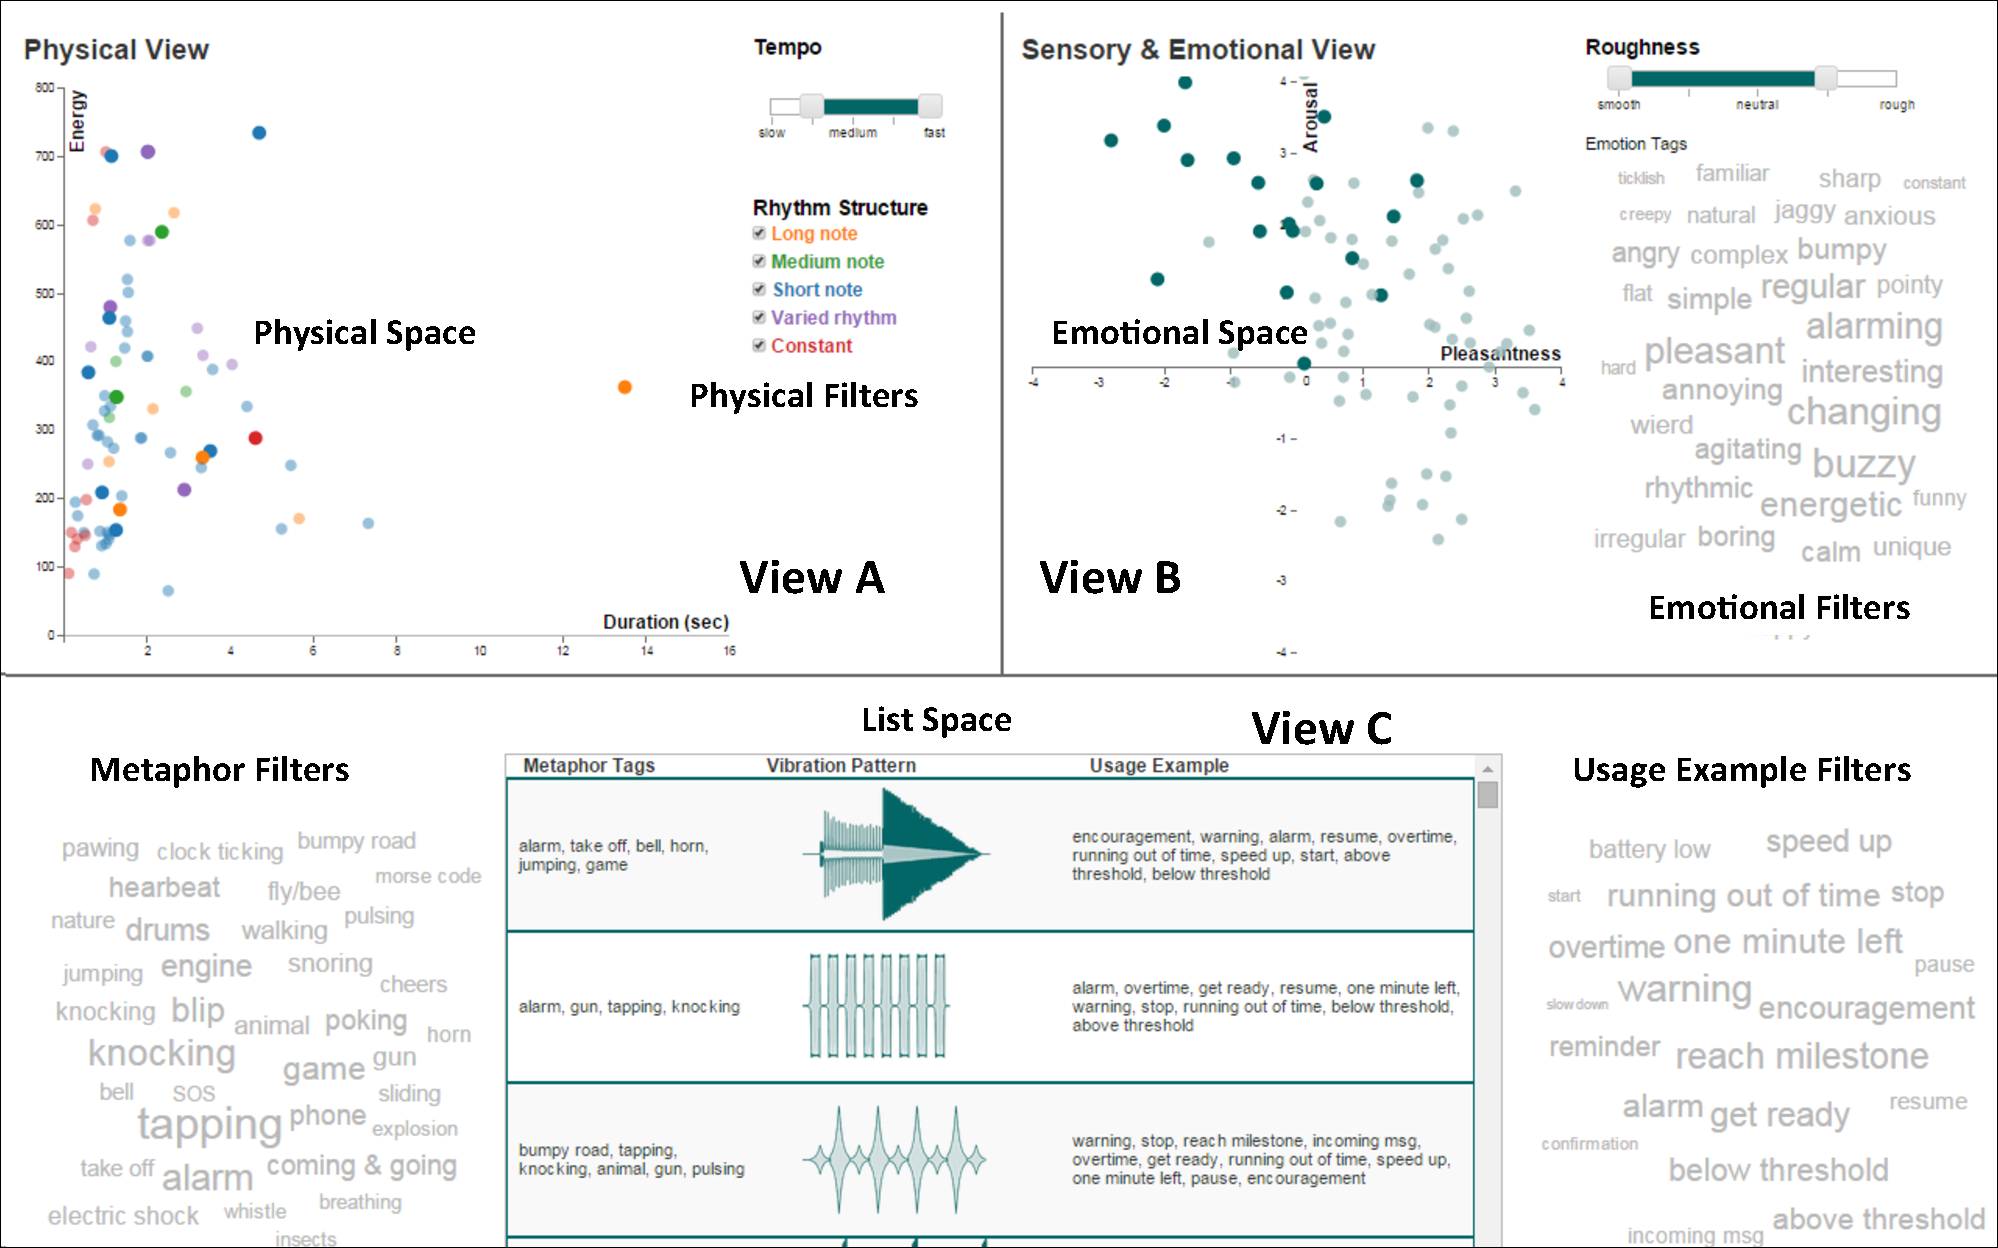
\includegraphics[width=\textwidth, height=1.2in]{VibViz-Screenshot}
            \caption{VibViz interface ~\cite{Seifi2015}}
            \label{fig:vibviz}
         \end{subfigure}~
	\begin{subfigure}{0.19\textwidth}
    	\centering
     	 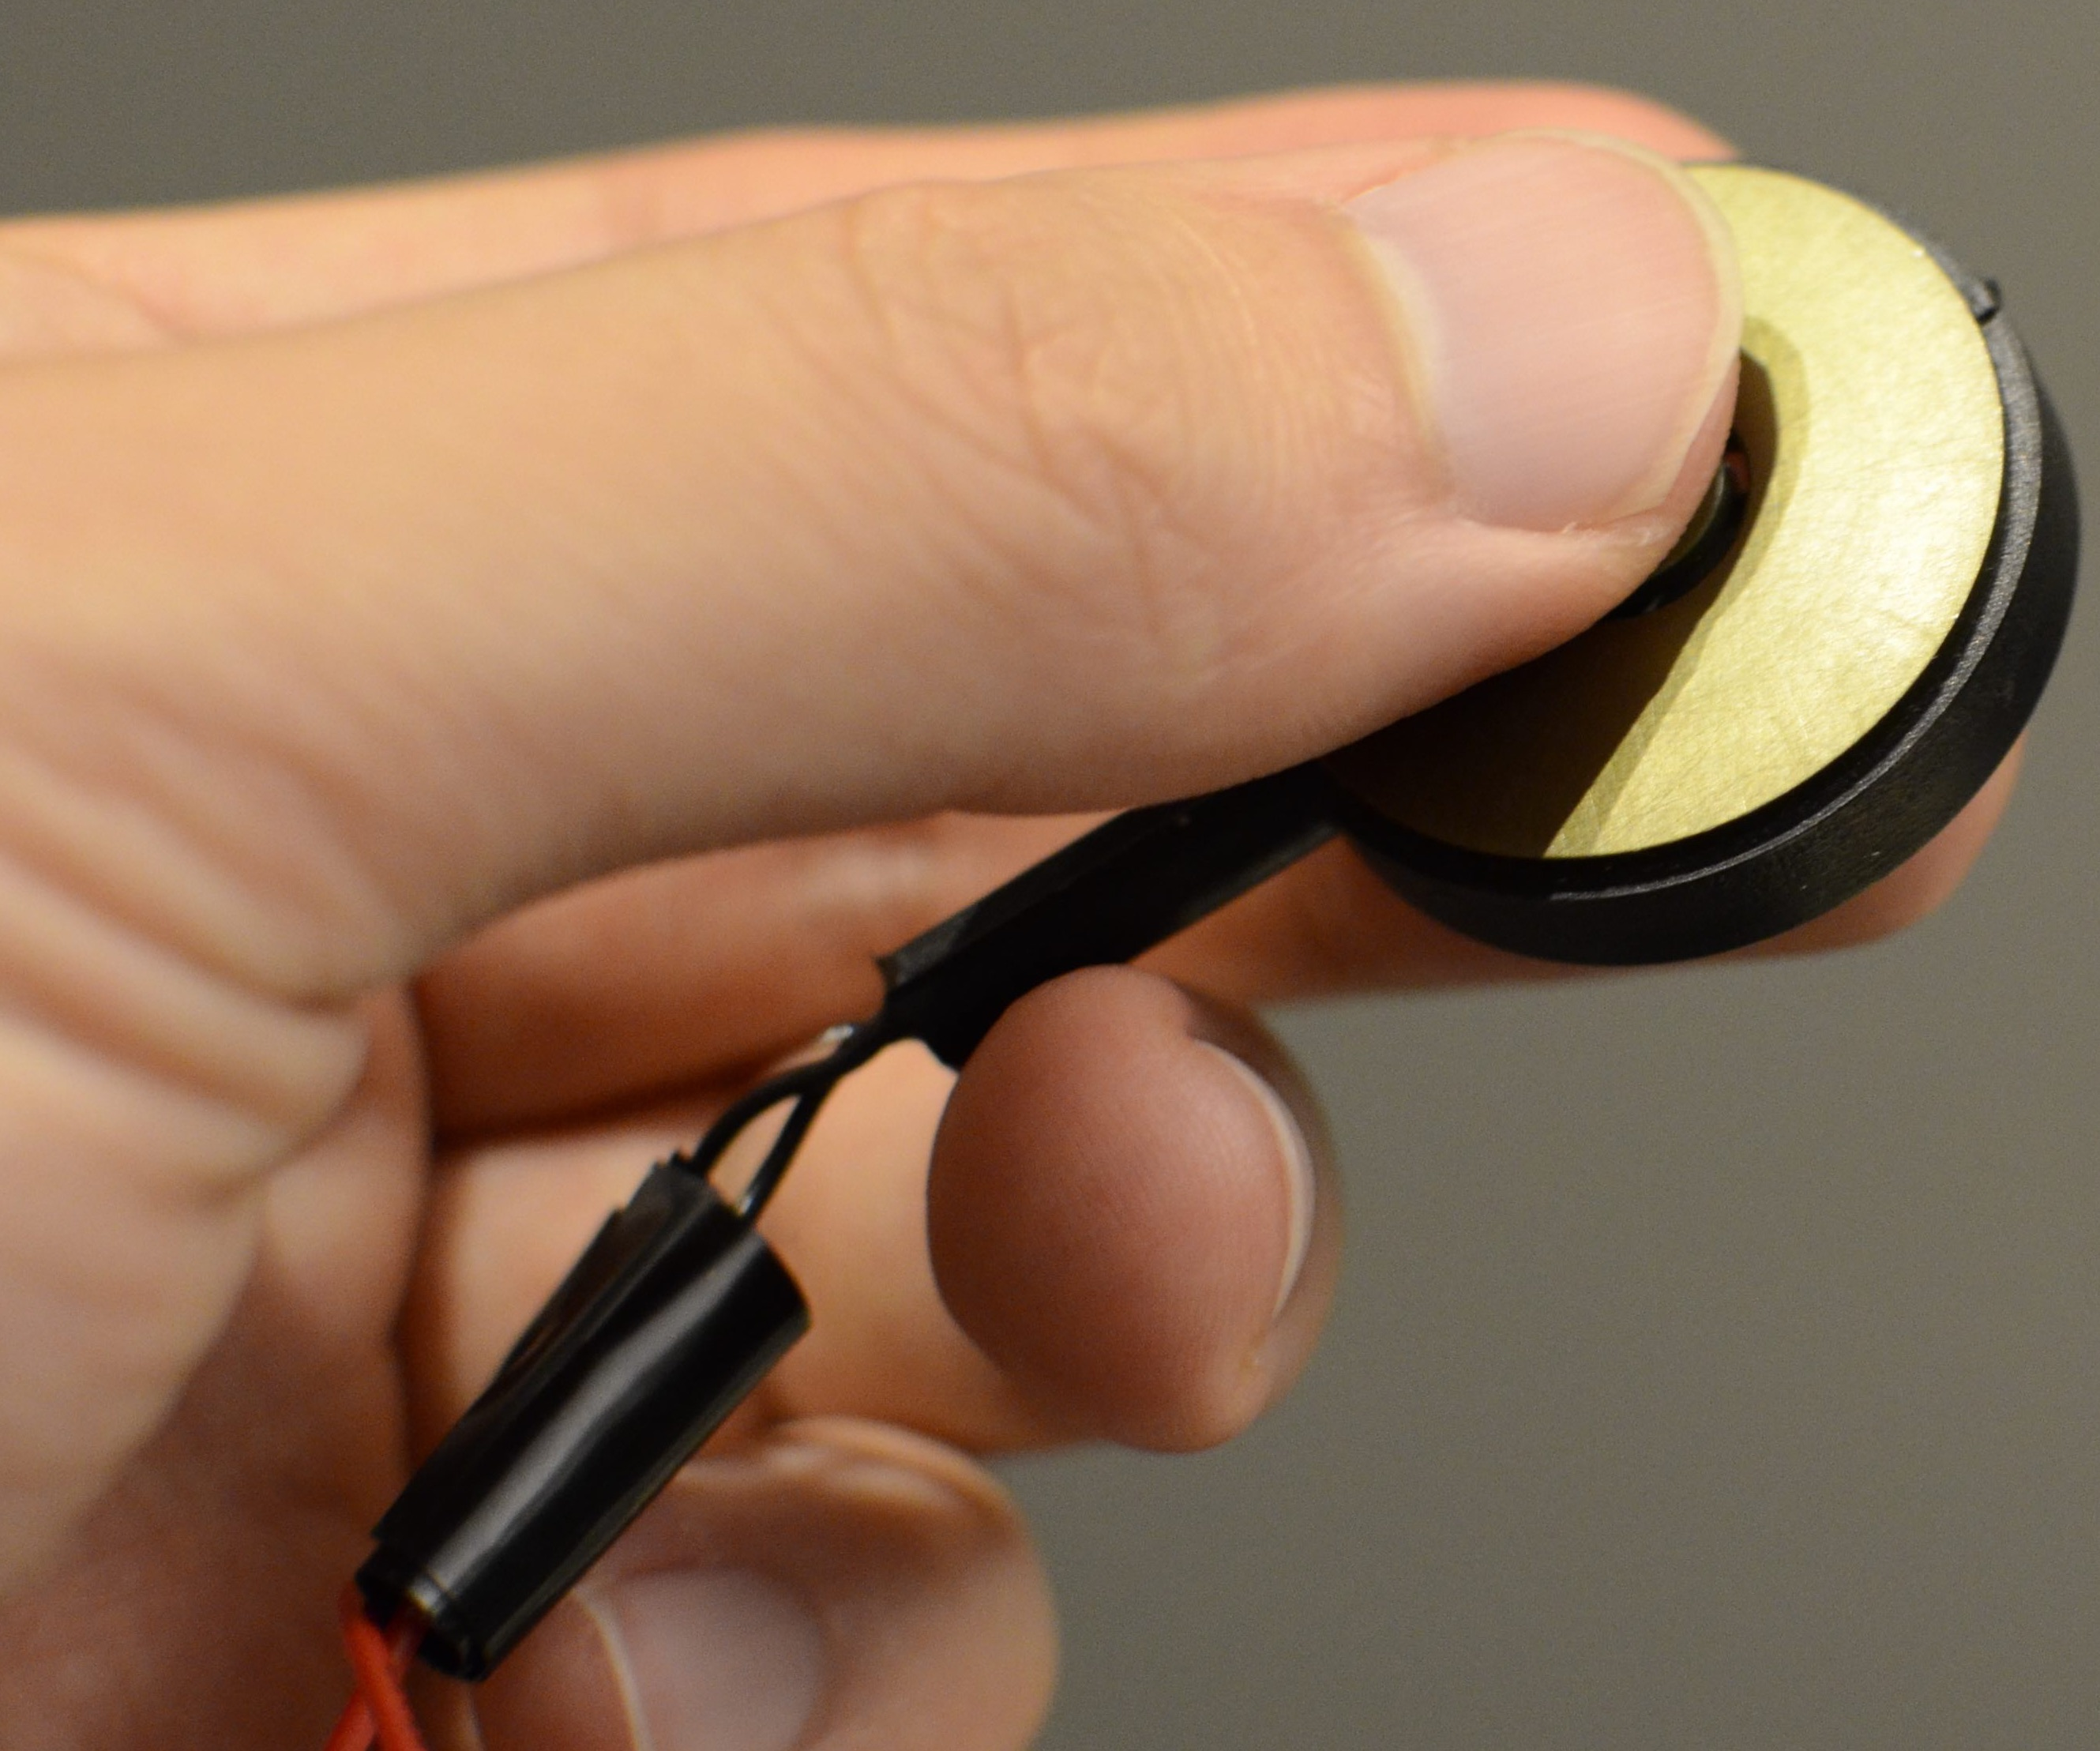
\includegraphics[width=\textwidth, height=1.2in]{C2-Tactor-Held2}
            \caption{C2 tactor}
            \label{fig:c2tactor}
         \end{subfigure}
            \label{fig:approach}
            \caption{Source of high-fidelity vibrations and perceptual rating scales.}
\end{figure}

\vspace{0.25in}
\section{Sourcing reference vibrations and qualities}% and qualities}
%\section{Approach \kmE{for Proxy Design and Validation} }
%\kmC{Approach for whole paper, or just  proxy design? SLC}
% If just proxy design (all that's covered in section currently), title section appropriately.
% If for whole paper, Start by overviewing entire approach, don't jump in piecemeal. Then, add sections for the rest - e g. validation process. 
% SUGGEST: Approach for Proxy Design and Validation.  ADD: a subsection, perhaps at start, outlining how you plan to validate (series of studies, what their goals are and how they build on one another. What's the logic?)

%\kmC{SLC: algorithm?} % after reading the Vis and Lofi sections, I'm not confident how streamlined the translation process is. It's okay if it isn't, but need to address this here if so. Say that we're doing a feasibility study, aimed to figure out how the translation should work, so its premature for automoation. HOWEVEr, it is a must that it follows a consistent set of heuristics that COULD be mechanized. }

We required a set of exemplar source vibrations on which to base our proxy modalities. 
This set needed to
1) vary in physical, perceptual, and %affective
emotional characteristics,
2) represent the variation in a larger source library, and
3) be small enough for experimental feasibility.


\subsection{High-fidelity reference library}
We chose 10 vibrations from a large, freely available library of 120 vibrations (VibViz, \cite{Seifi2015}), browsable through five descriptive taxonomies, and ratings of taxonomic properties. Vibrations were designed for an Engineering Acoustics C2 tactor, a high-fidelity, wearable-suitable voice coil, commonly used in haptic research~\cite{Seifi2015}.
We employed VibViz's filtering tools to sample, ensuring variety and coverage by selecting vibrations at  high and low ends of energy / duration dimensions, and filtering by ratings of temporal structure/rhythm, roughness, pleasantness, and urgency.
To reduce bias, two researchers independently and iteratively selected a set of 10 items each, which were then merged.

Because VibViz was designed for a C2 tactor, we used a handheld C2 in the present study (\autoref{fig:c2tactor}).

       \begin{figure}
        \centering
        \begin{subfigure}{0.15\textwidth}
            \centering
            
\includegraphics[width=\textwidth]{v-09-09-8-24}
        \end{subfigure}
        \begin{subfigure}{0.15\textwidth}
            \centering
            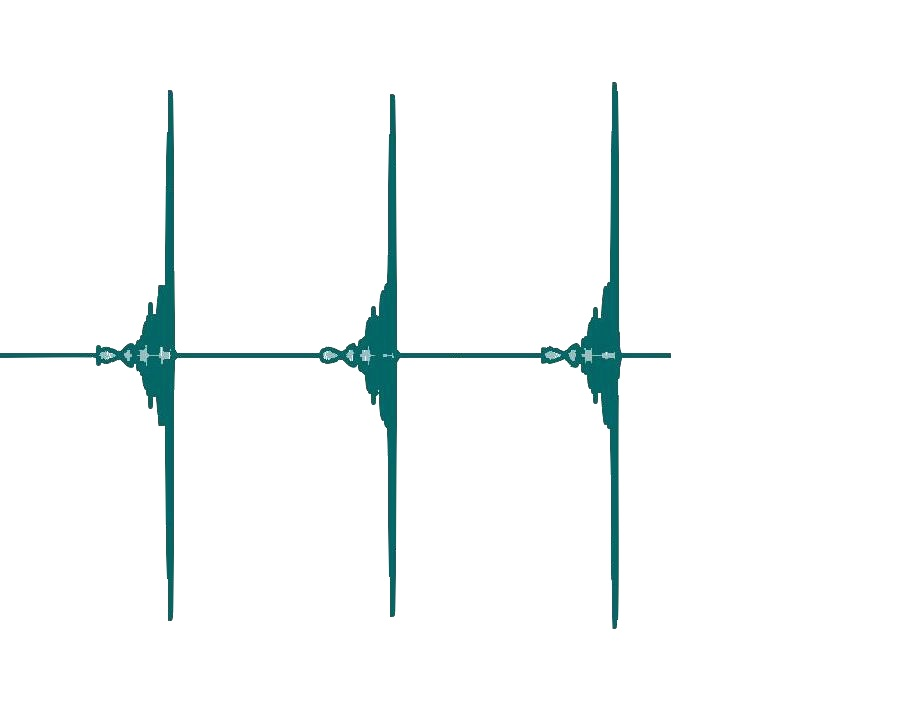
\includegraphics[width=\textwidth]{v-09-10-7-34}
        \end{subfigure}
        \begin{subfigure}{0.15\textwidth}
            \centering
            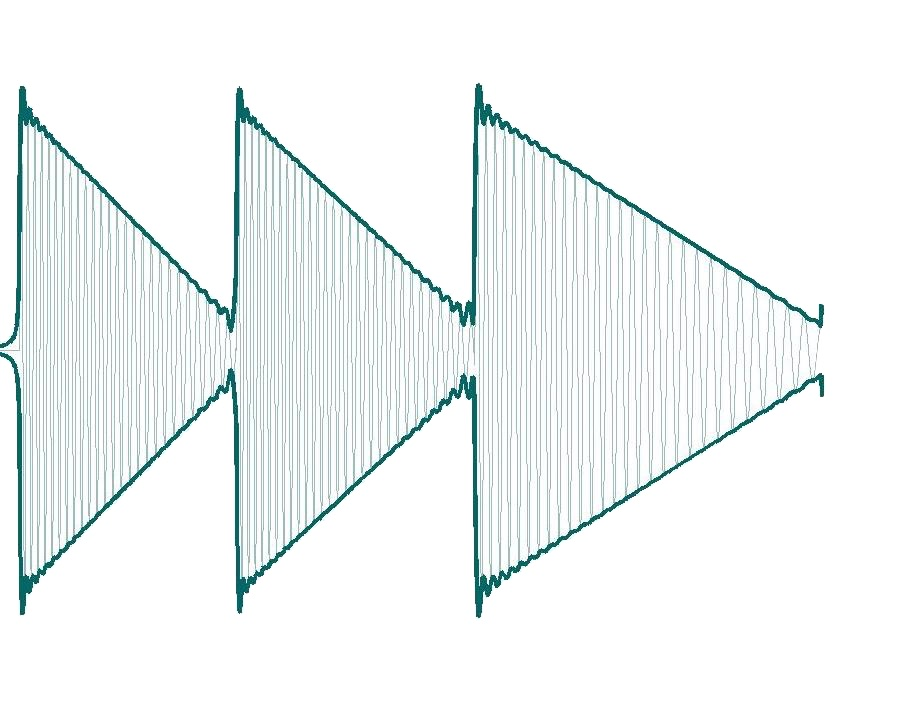
\includegraphics[width=\textwidth]{v-10-21-3-11}
        \end{subfigure}
        \caption{\original~Visualization, based on VibViz}
        \label{fig:vis:original}
    \end{figure}

\subsection{Affective properties and rating scales} 
To evaluate our proxies, we adapted six rating scales from the tactile literature and new studies.
%
Seifi \etal~\cite{Seifi2015} proposed five taxonomies for describing vibrations including  physical, sensory, emotional, metaphors, and use examples.
Three taxonomies comprise quantitative metrics and adjectives; two use descriptive words. 

We chose six quantitative metrics from \cite{Seifi2015} that capture important affective (physical, perceptual, and %affective
emotional) VT qualities:
%\kmC{HASTI, can you include the ranges for these? %low/hi, long/short, smooth/rough?
 1) \textit{duration} [low-high], 
 2) \textit{energy} [low-high], 
 3) \textit{speed} [slow-fast], 
 4) \textit{roughness} [smooth-rough], 
 5) \textit{urgency} [relaxed-alarming], and 
 6) \textit{pleasantness} [unpleasant-pleasant].
A large scale (0-100) 
%, compared to more common 5 or 7 point scales)
allowed us to treat the ratings as continuous variables.
To keep trials quick and MTurk-suitable,
%(especially when deploying over MTurk), 
we did not request open-ended responses or tagging. %what kind of tagging?

\section{Proxy Choice and Design}
%: Capturing higher-level traits}
The proxies' purpose was to capture high-level traits of source signals. 
We investigated two proxy channels and approaches, \magenta{to efficiently establish viability and search for triangulated perspectives on what will work.} % while limiting scope to two. 
The most obvious starting points are to 
1) visually augment the current standard of a direct trace of $amplitude=f(time)$, and
2) reconstruct vibrations for common-denominator, low-fidelity actuators.

We considered other possibilities (e.g., auditory stimuli, for which MTurk  has been used~\cite{Cartwright2015}, \magenta{or animations). 
However, our selected modalities balance
a) directness of translation (low fidelity could not be excluded);
b) signal control (hard to ensure consistent audio quality/volume/ambient masking); and
c) development progression (visualization underlies animation, and is simpler to design, implement, display).
We avoided multisensory combinations at this early stage for clarity of results. Once the key modalities are tested, combinations can be investigated in future work.}  



%\kmC{SLC - nonspace?} % Can you briefly talk about the non-space? Were these the only two possibilities that could possibly be considered? Eg., why not Audio? 


    \begin{figure*}
        \centering
        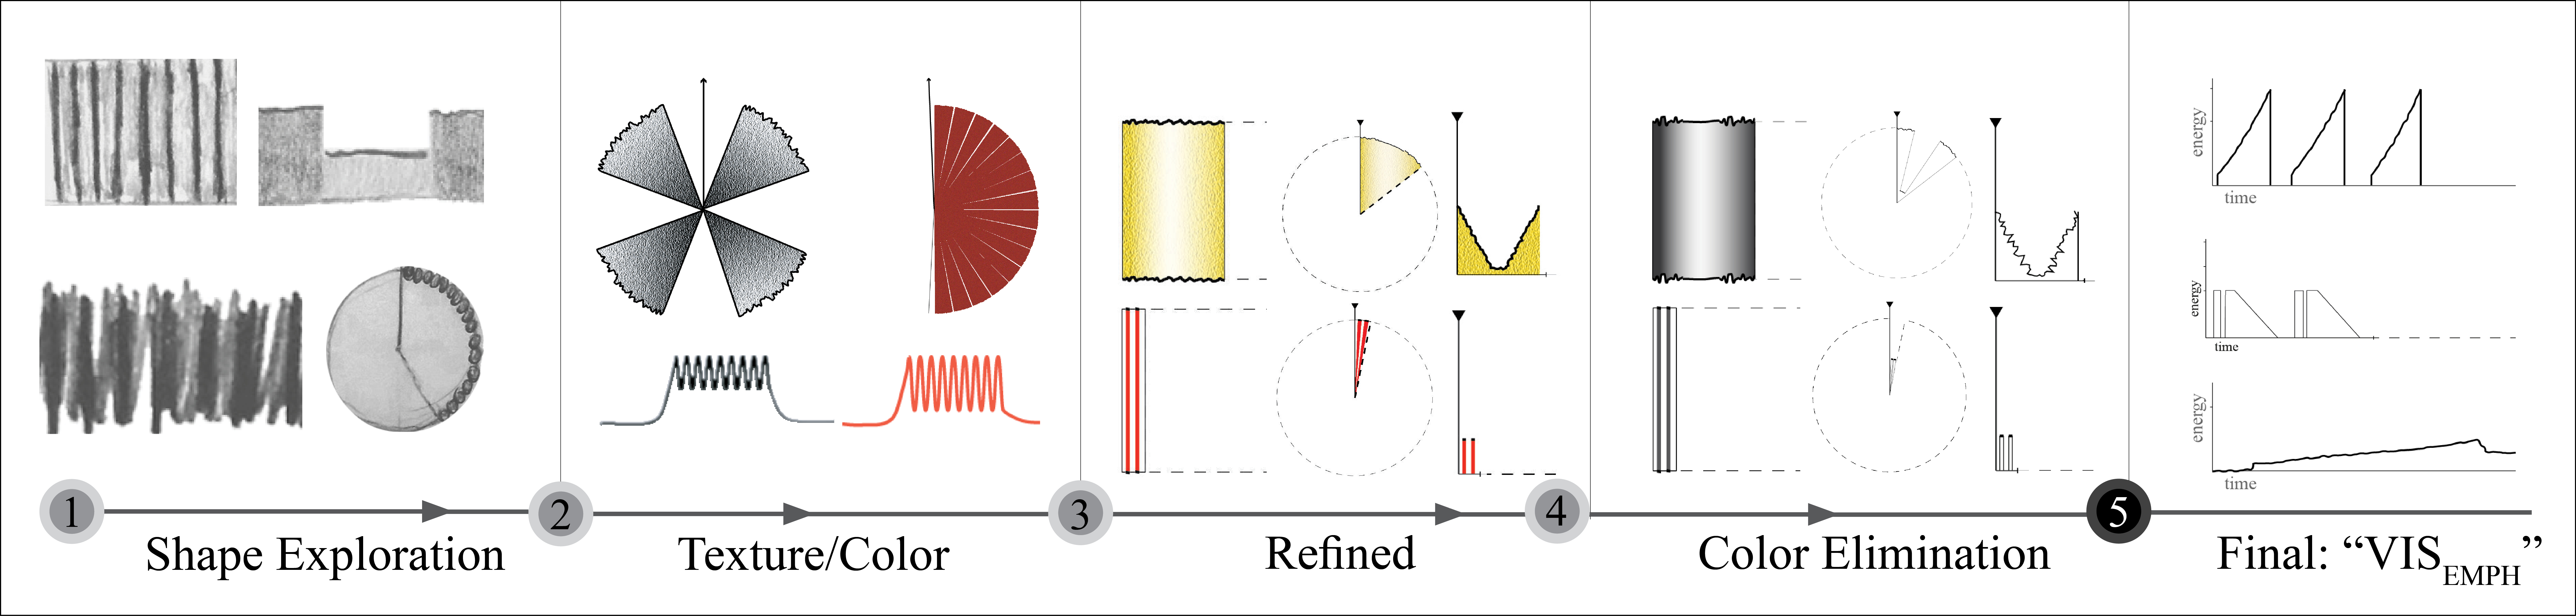
\includegraphics[width=\textwidth]{Figure4(1200res)}
        \caption{Visualization design process. Iterative development and piloting results in the \linear~visualization pattern.}
        \label{fig:vis:initialdesigns}
    \end{figure*}
    
        \begin{figure*}
        \centering
                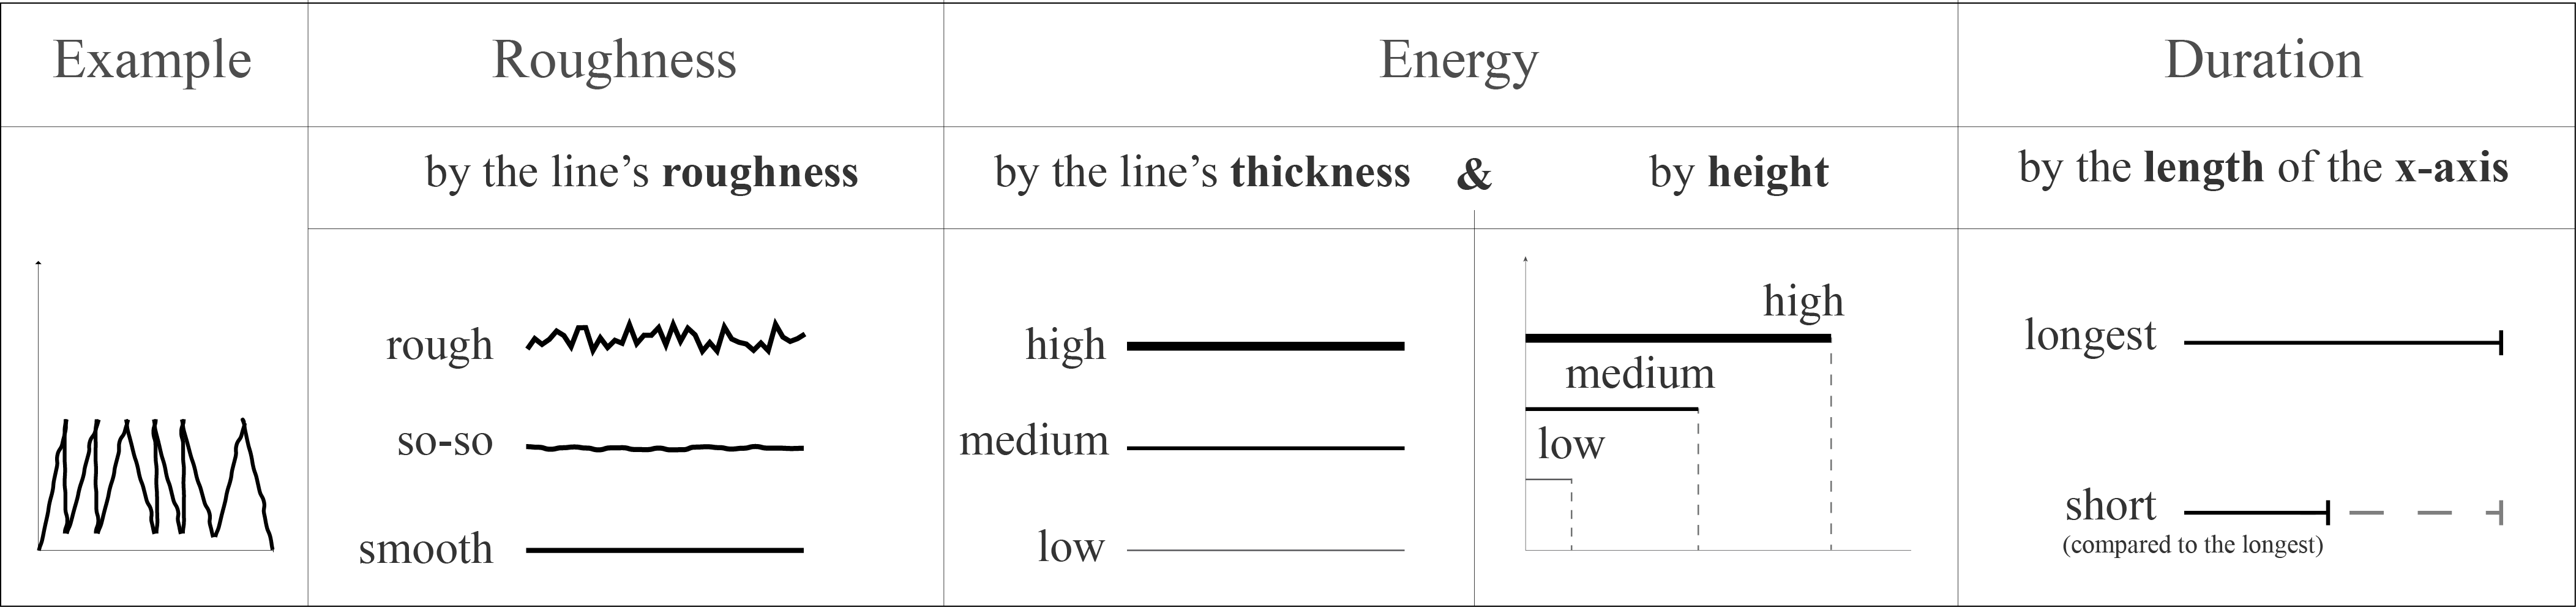
\includegraphics[width=\textwidth]{Guideline-GRPH-EMPH}
                \caption{Final \linear~ visualization guide, used by researchers to create \linear~proxy vibrations and provided to participants during \linear~study conditions.}
            \label{fig:vis:ref:guideline}
    \end{figure*}

``\hifi" denotes high-fidelity source renderings (C2 tactor).

\textbf{1)	Visual proxies:} 
% The visual proxy for vibrations was inspired by the extensive use of vibration waveforms in VT design.
Norms in published works (e.g. \cite{Chan2008}) directed~\cite{Seifi2015} to confirm that users % find  utility in and 
rely on graphical $f(time)$ plots to skim and choose from large libraries.  We tested the direct plot, \original, as the status-quo representation.

However, these unmodified time-series emphasize or mask traits differently than felt vibrations, in particular for higher-level or ``meta" responses. %interpretations.
We considered many other means of visualizing vibration characteristics, pruned candidates and refined design via piloting to produce a new scheme which explicitly \textit{emphasizes} affective features, \linear.


\textbf{2)	Low-fidelity vibration proxy:} 
Commodity device (e.g. smartphone) actuators usually have low output capability compared to the C2, in terms of frequency response, loudness range, distortion and parameter independence. Encouraged %by work on translating audio \cite{Lee2013} and video \cite{Kim2014} to haptics, and 
by expressive rendering of VT sensations with commodity actuation (from early constraints~\cite{Chan2008} to deliberate design-for-lofi~\cite{Israr2015}), we altered stimuli to convey high-level parameters under these conditions,
hereafter referred to as \lofi.

% Next, we describe our development of the \original, \linear, and \lofi~proxy vibrations in more detail.
\textbf{Translation:} 
Below, we detail first-pass proxy development.
In this feasibility stage,  we translated proxy vibrations manually and iteratively, as we sought generalizable mappings of the parametric vibration definition to the perceptual quality we wished to highlight in the proxy. We frequently relied on a cycle of user feedback, e.g., to establish the perceived  roughness of the original stimuli and proxy candidate. 

Automatic translation is an exciting goal. Without it, HapTurk is still useful for gathering large samples; but automation will enable a very rapid create-test cycle. 
%We believe
It should be attainable, bootstrapped by the up-scaling of crowdsourcing itself. With a  basic process in place, we can use MTurk studies to identify these mappings relatively quickly.

\vspace{0.25in}

\subsection{Visualization Design (\original\ and \linear)}
%We used two visualization methods as proxies: \original, a typical waveform-based visualization, and \linear, specifically designed to convey our high-level perceptual 
%%Here we describe our process for developing both.
%%\original~ is an adaptation of VibViz's waveform method to include a vibration duration and scaled amplitude, to provide a baseline for existing visualization methods.
%% \linear~was iteratively developed to depict our 6 high-level qualities.

    \original\ was based on the original waveform visualization used in VibViz  (\autoref{fig:vis:original}).
%    \kmC{SLC} % this is confusing. You say it's based on VibViz, describe the encoding It hink for VibViz, say that was bad and we did something different here. So, how is it based on VibViz?
    In Matlab, vibration frequency and envelope were encoded to highlight its pattern over time.
    Since \original\ patterns were detailed, technical and often inscrutable for users without an engineering background, we also developed a more interpretive visual representation,  \linear; and 
    included \original\ as a status-quo baseline.

    
      %In the VibViz study, 5 initial taxonomies including (1) physical characteristics (e.g., duration, energy), (2) sensory characteristics (e.g., roughness), (3) emotional characteristics (e.g., pleasantness, arousal), (4) usage examples (e.g., reminder), and (5) metaphors (e.g., snoring), were used for describing vibrations.
    %A subset of these taxonomies was for the visualizations. Due to the challenging nature of illustrating usage example and metaphor characteristics through simple waveforms, only the physical, sensory and emotional characteristics were selected for this stage of the study.
    
    
%    \subsection{Initial exploration}
  
  %
  %Process: Going from stage 1 to 3 it was mainly us. Going from 3 to 4, I talked to 4 other people (my friends and lab-mates). Stage 4 to 5, I did a survey with 7 participants, again friends and family.
  %
%  \kmC{SLC: tighten} % don't need this much detail, and it is a very long para. (I broke it into two)
%  \kmC{I am not getting a sense of a translatory ``algorithm''. Is there one?}
  We took many approaches to depicting vibration high-level properties, with visual elements such as line thickness, shape, texture and colour (\autoref{fig:vis:initialdesigns}).
    %were developed to test the accuracy of the mappings between vibrations and their visuals.
        We first focused on line sharpness, colour intensity, length and texture:
        graphical waveform smoothness and roughness were mapped to perceived roughness; 
        colour intensity highlighted  perceived energy.
        Duration mapped to length of the graphic, while colour and texture encoded the original's invoked emotion.
%        This exploration resulted in the development of 3 different proposed patterns (linear, circular and rectangular, \autoref{fig:vis:proposed}).

    % After developing a set of visualization candidates, 
    Four participants were informally interviewed and asked to feel \hifi~vibrations, describe their reactions, and compare them to several visualization  candidates.
         Participants differed in their responses, and  had difficulties in understanding VT emotional characteristics from the graphic (i.e. pleasantness, urgency), and in reading the circular patterns. 
       We simplified the designs, eliminating representation of emotional characteristics (color, texture), while retaining more objective mappings for physical and sensory characteristics. % \affect{in our proxy design}.
       % \affect{I don't understand the previous sentence. Does it mean that we did not focus on emotional characteristics in our design, but still evaluated these characteristics ?!} 
       
       \linear~won an informal evaluation of final proxy candidates (n=7), and was captured in a translation guideline
       % for translating a \hifi~vibration to a \linear~proxy 
       (\autoref{fig:vis:ref:guideline}).
     
    
     
%        As a first set of visualizations, original waveform patterns of the 10 selected vibrations are scaled and represented on a 2-dimensional graph with time on the x-axis and amplitude on the y-axis.
%        The linear patterns are selected as the second set. They are designed using a basic guideline that translated the main characteristics of a vibration such as roughness, energy and duration (\autoref{fig:vis:ref:guideline}, \autoref{fig:vis:ref:comparison}). 
%        The guideline highlights that the line'??s thickness corresponds to energy level of the vibrations.
%        For easy comprehension of the patterns, the energy and roughness levels of the vibrations are divided into 3 ordinal groups: low, medium and high.
%        Roughness is highlighted through the smoothness or sharpness of the waveforms.
%        In addition to the line'??s thickness, energy level is also highlighted on the y-axis on the linear pattern graphs.
%        The x-axis displays time.
%        Duration of the vibration is displayed with a solid line and as a point of reference; the duration of the longest vibration is displayed on the same graph with a dashed line.
        

   

\subsection{Low Fidelity Vibration Design} 
%In addition to visualization proxies, 
For our second proxy modality, we translated \hifi~vibrations into \lofi~vibrations.
We used a smartphone platform for their built-in commodity-level VT displays, their ubiquity amongst users, and low security concerns for vibration imports to personal devices~\cite{Felt2012}.
To distribute vibrations remotely, we used HTML5 Vibration API, implemented on Android phones running compatible web browsers (Google Chrome or Mozilla Firefox).

%\kmC{SLC: algorithm?} % as for visual - need to hear the automatable algorithm or process.
As with \linear, we focused on physical properties when developing \lofi (our single low-fi proxy exemplar).
We emphasized rhythm structure, an important design parameter \cite{Ternes2008} and the only direct control parameter of the HTML5 API, which issues vibrations using a series of on/off durations.
%%%%%%%
Simultaneously, we manipulated perceived energy level by adjusting the actuator pulse train on/off ratio, up to the point where the rhythm presentation was compromised.
%%%%
%As defining the vibration motor time durations was the main method to create vibrations, this was by far the biggest limitation to overcome. The time durations controlled the overall energy felt by the phone and the general rhythm (on/off beats).
Shorter durations represented a weak-feeling hi-fi signal, while longer durations conveyed intensity in the original.
%But with these limitations in mind, an initial set of 10 lower fidelity vibrations were created.
%
% \subsection{Design Process}
 %
% Our general process in creating these low-fi vibrations were to adjust the various ?on? segments of the original vibration in their timings to match their energy levels, while adjusting the ?off? motor times to represent the necessary pauses of the vibration?s rhythm structure.
%    
%Representing accurate rhythm structure was straightforward for the candidate vibrations that contained short vibration segments with consistent energy levels. These sorts of vibrations required timing the ?on? motor times to match their original counterparts energy levels - often short time durations of around 50 to 100 ms. The ?off? time durations closely matched the original vibrations off times to match the rhythm. 
%
This was most challenging for dynamic intensities or frequencies, such as increasing or decreasing ramps, and long, low-intensity sensations.
Here we used a duty-cycle inspired technique, similar to \cite{Israr2015}, illustrated in \autoref{fig:vib:lofidesign}.
%\kmC{SCOPE NOTE - SLC} % This is another important scope limitation that you may need to highligyt in Intro / Approach. This limitation is kind of sidestepping the broad claim of crowdsourcing. So you need to explain that it allows you to ACCESS crowdsourcing,but need to limit that pool to subjects that have this kind of phone. This is still pretty good! However, it raises the question of verifying compliance.}
%

To mitigate the effect of different actuators found in smartphones, we limited our investigation to Android OS.
While this restricted our participant pool, there was nevertheless no difficulty in  quickly collecting data for either study.
We designed for two phones representing the largest classes of smartphone actuators: Samsung Galaxy Nexus, which contains a coin-style actuator, and a Sony Xperia Z3 Compact, which uses a pager motor resulting in more subdued, smooth sensations.
Though perceptually different, control of both actuator styles are limited to on/off durations.
As with \linear, we developed \lofi~vibrations iteratively, first with team feedback, then informal interviews (n=6).

% vibration segments in their energy levels, this process was trickier. These vibrations often featured the escalation of energy over a vibration?s on segments. To emulate this, we had to carefully pick the initial ?on? time and increase this time with appropriate time increments as well as making sure the ?off? times decreased in parallel to allow for the peak energy levels to be felt though the longer motor ?on? times. An example of this type of vibration would be {\tt [1,77,2,76,3,75, ...., 77,1] }showing that the ?on? motor times gradually increase while the ?off? times decreases. 
%\subsection{Feedback on initial low fidelity vibration designs}

%We primarily verified these low-fi vibrations on a Samsung Galaxy Nexus, which incorporated a ?coin? vibration motor. These motors resulted in creating ?textured? vibrations resembling the energy levels of the original vibrations. Our other test phone was the Sony Xperia Z3 Compact, which used an ?pager? vibration motor. By comparison, these motors felt subdued and smoother. Early design reviews indicated the initial vibrations designed for the Samsung phone felt much more weaker than on the Sony phone, due to the different vibration motors used by each. The differences in the felt vibrations among these motors requires an explanation of their characteristics. 
%    Ref:
%    Vibration Motor Differences
%http://www.precisionmicrodrives.com/vibrating-vibrator-vibration-motors/pancake-shaftless-coin-vibration-motors/design-considerations)

%``Pager" vibration motors can be thought of as the most basic form of a vibration motor, essentially a DC motor with an small offset mass attached to a rotating shaft. When the offset mass is rotated, this causes a repeated displacement of the whole motor that is perceive as a vibration. ?Coin? vibration motors are similar in that it uses a rotating disc mass that is located inside a metal case enclosure. The disc mass rotates via magnetic field interactions, causing the entire coin-shaped motor to vibrate. 

%By comparison, the ``coin" vibration motors vibrate a larger area of motors compared to the more compact coverage of ``pager" motors, which may contribute to the more intense feeling of these motors.?Coin? motors also require a relatively higher start voltage to begin the vibration process compared to ?pager? vibration motors. This may also contribute to a ?harder? vibration feeling than ?pager? motors that require lower voltages to continue vibrating [ref]. 


%
%Based on team feedback, all of our low-fi vibrations were adjusted to accommodate both types of vibration motors in these phones, to accommodate as much motor variety among different phone brands as seen from these phones. The goal was to maintain the rhythm of the vibratins to be as similar as possible on both phones while imparting as much energy from their respective motor types. 
    
    \begin{figure}
        \centering
        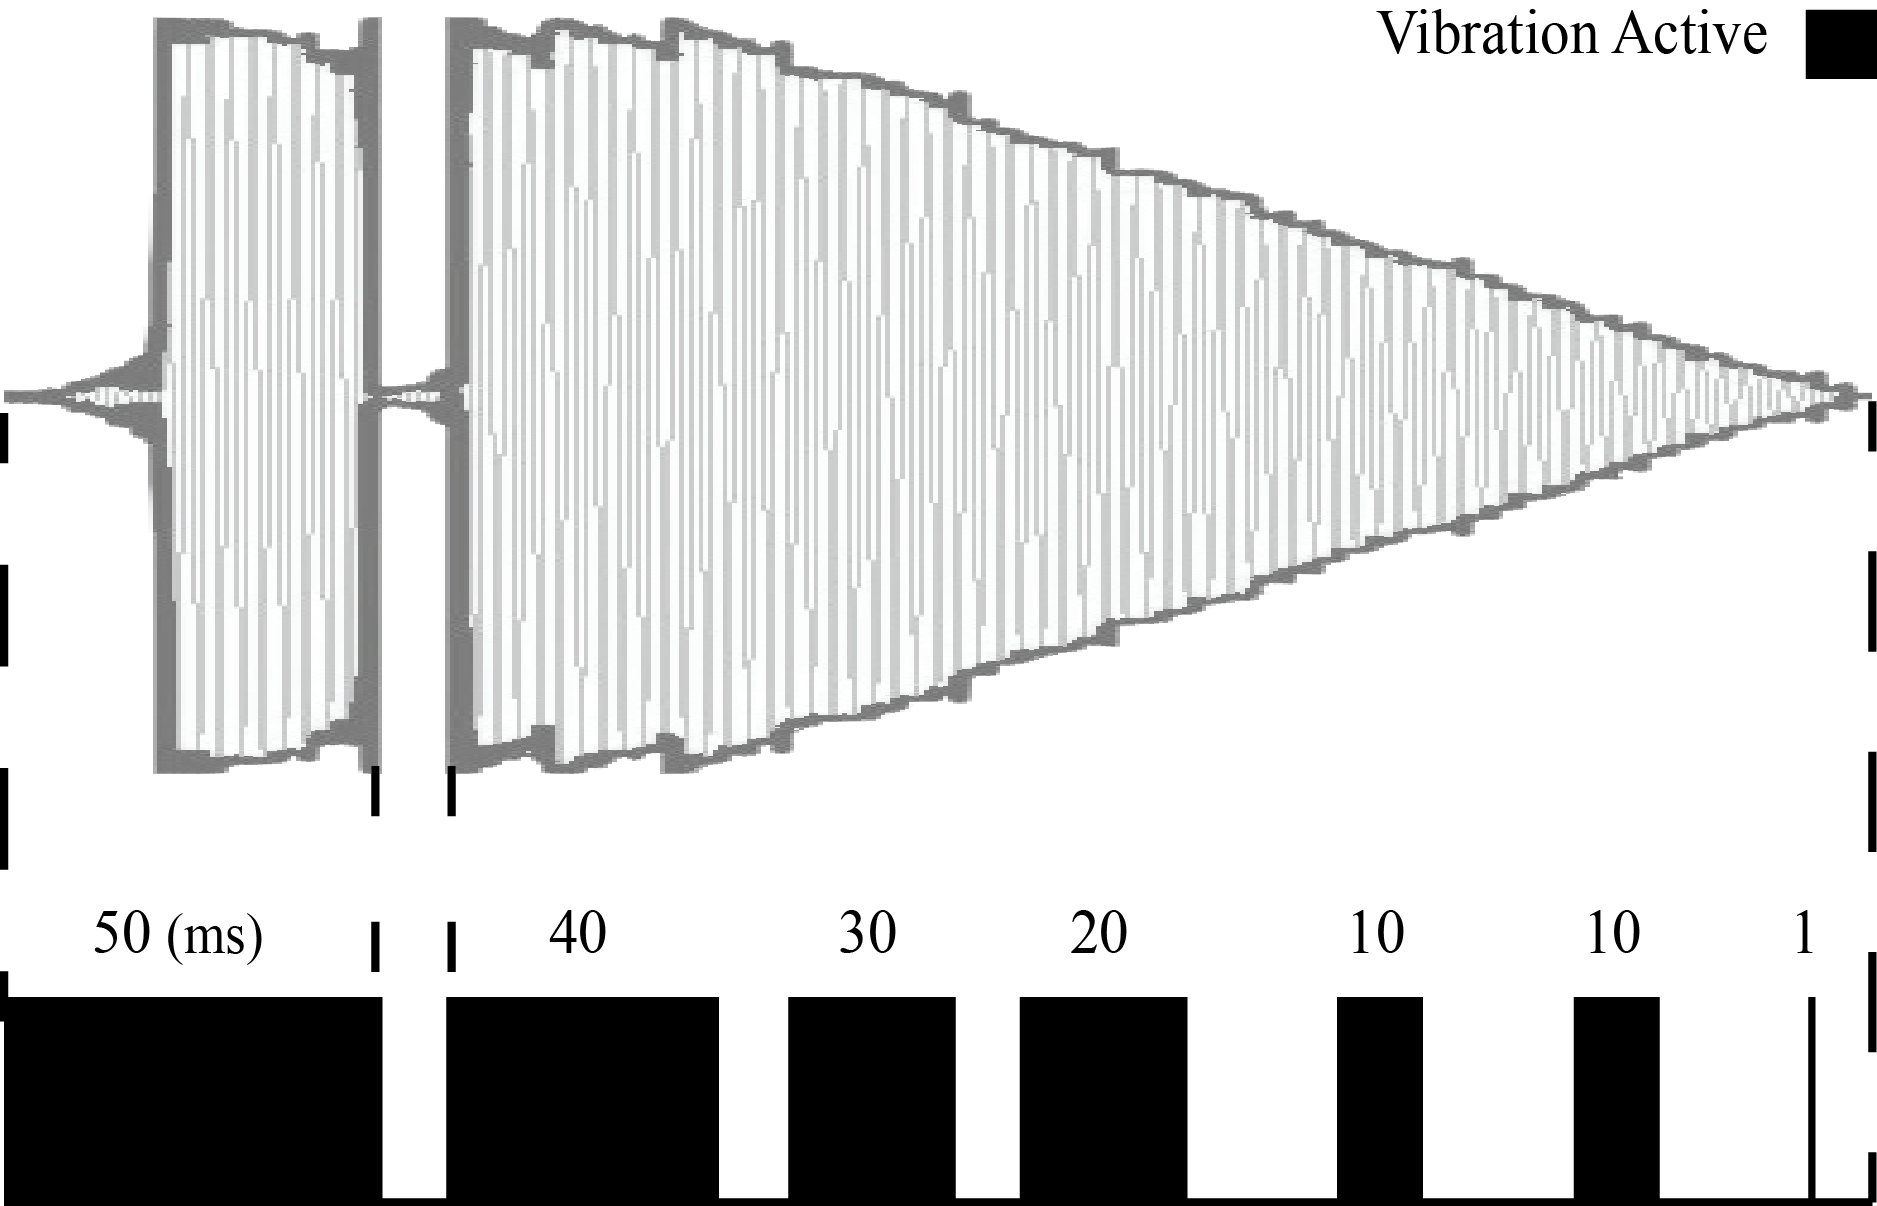
\includegraphics[width=0.42\textwidth, height=1.65in]{VibratorTime}
        \caption{Example of \lofi\ proxy design. Pulse duration was hand-tuned to represent length and intensity, using duty cycle to express dynamics such as ramps and oscillations.}
        \label{fig:vib:lofidesign}
    \end{figure}

 
    \begin{figure*}
        \centering
                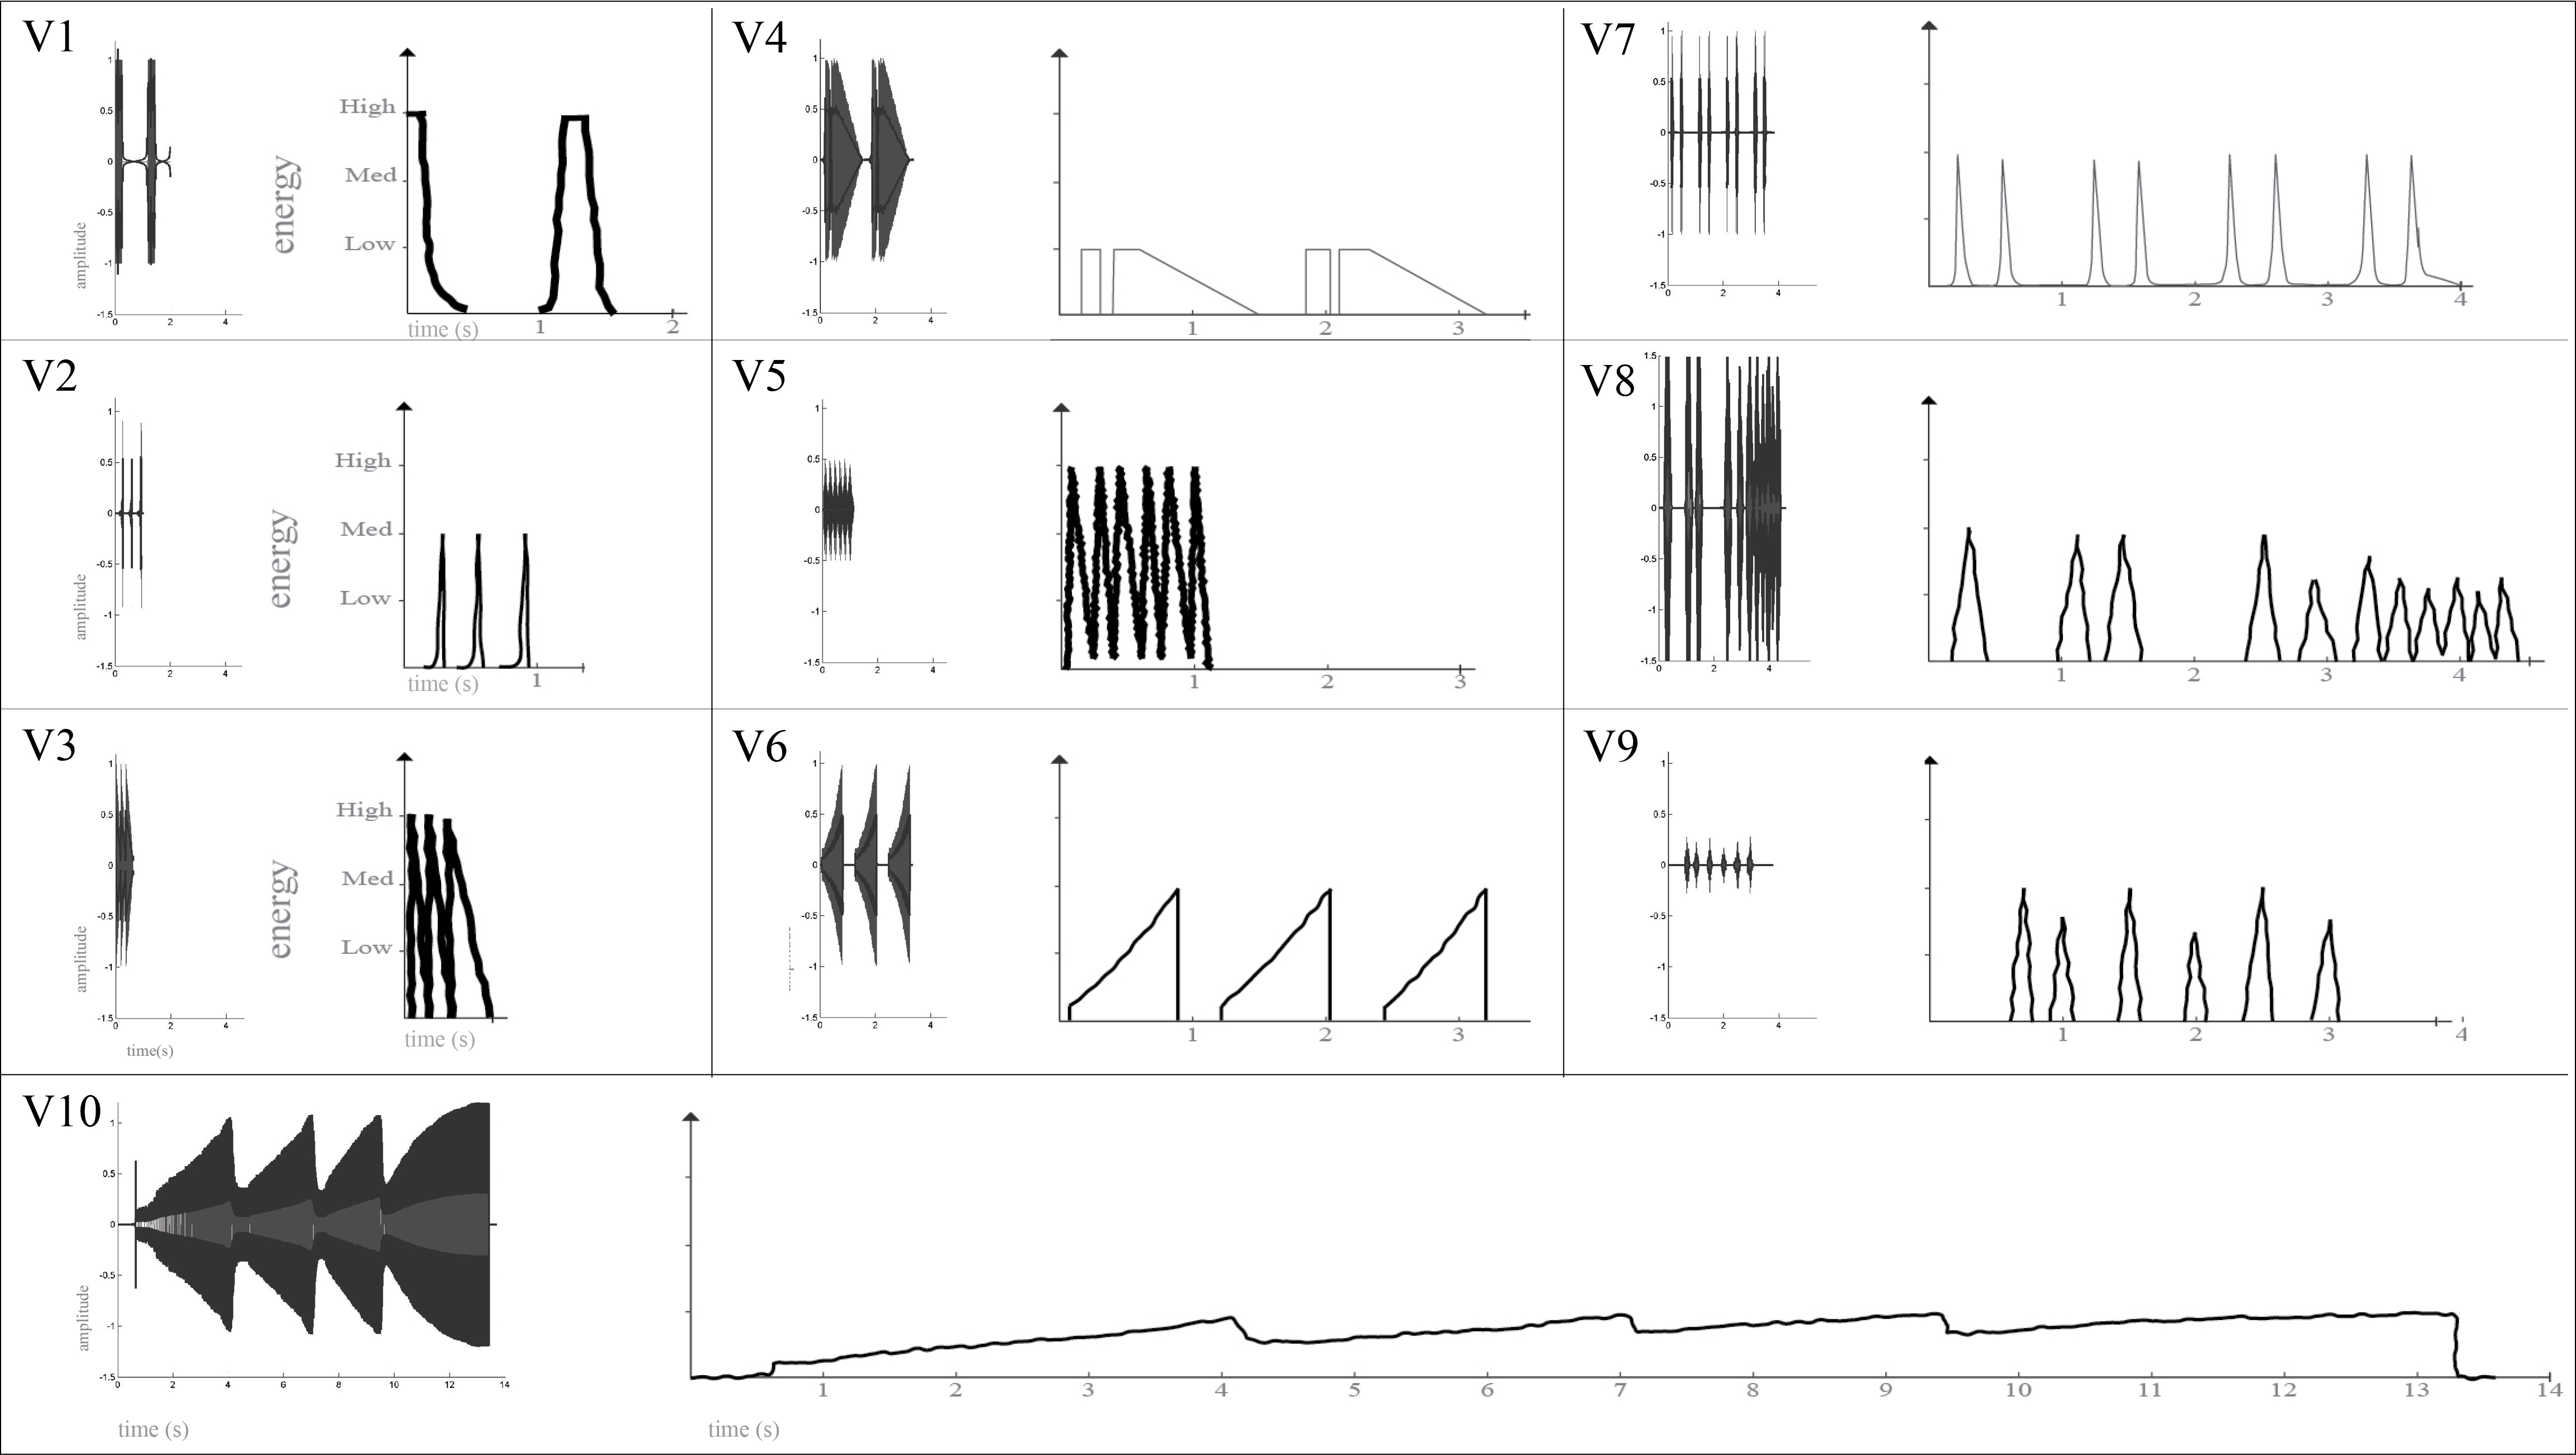
\includegraphics[width=\textwidth]{AllVISNewNumbering}
                \caption{Vibrations visualized as both \original\ (left of each pair) and \linear.}
            \label{fig:vis:ref:comparison}
        \end{figure*}



%\subsection{Final low fidelity vibration designs}    
%    After many iterations with fellow team members, the final version of the low fidelity vibrations were deemed appropriate in capturing the "essence" of the original vibrations. These vibrations were further verified through pilots employing custom web surveys on various  mobile web browsers. This was to check for any technical problems. It was found that the vibrations were playable on the expected hardware and web browsers to be used.
    


%    were recruited through the university graduate and undergraduate mailing lists. Participants were not exposed to the other vibrotactile study.
%    Conditions - We were comparing  ratings of different metrics between visual and vibotactile representations of the vibrations. We compared ratings on 6 metrics: 
%    1. Speed (beat/second)
%    2. Duration
%    3. Energy
%    4. Roughness
%    5. Pleasantness
%    6. Urgency
%     
%    Tasks - Participants were asked to complete three surveys. Two of the surveys included visual representations of the vibrations. The third survey was designed for the vibrotactile stimuli. For the linear visual design survey, participants were presented with a guideline to help them with identifying vibration�??s physical properties such as duration, roughness and energy. They were then asked to complete the survey. With the vibrotactile survey, they were asked to play the vibrations on a second computer and feel the vibrations using the C2-tactor. 
%    
%    Design - Our experiment was a 3x10 repeated ANOVA test with 10 vibrations (between subjects) and 3 different representation methods (within subjects).
%    Factor 1: 10 Vibrations
%    Factor 2: Vibration presentation methods   a) Visual �?? Linear Pattern  
%    b) Visual �?? Original Pattern
%    c) Vibrotactile   
%    
%    Apparatus - We conducted the experiment in a laboratory at University of British Columbia. Two Windows laptop and an extra monitor were used. One monitor was used to display the survey. Another monitor was used to display the rules and the overview image of all the vibrations. The second laptop was used to access the vibrations. A C2-tactor device was connected to the second laptop for feeling the vibrations.
%    Independent and dependent variables
%    Independent variables: 1) Representation Method 2) Vibration  
%    Dependent variables: 1) Ratings of the 6 different metrics
%    Confounding variables: 1) C2-tactor 2) Individual differences
%    
%    Hypotheses
%    H1: There is no statistical significance between the average attribute scores obtained from the visual designs versus sensing the vibrotactile stimuli.
%    It is hypothesizes that the average attribute scores of at least one of the new sets is not significantly different from the original scores of the vibration obtained in VibViz study. In other words, the vibration�??s attributes that was obtained through visual representation correctly matches the ones obtained from physically sensing the vibrations.
%    H2: There is a statistical significance between the attribute scores of the linear visual pattern versus the original set.
%    
%    It is hypothesized that the new pattern will accurately represent vibrations�?? properties compared to the original patterns. In other words, the linear pattern will better visualize the vibrations for the users, compared to the original pattern.

%!!!!!!!!!!!!!!


\hspace{0.2in}
\section{Study 1: In-lab Proxy Vibration Validation (G1)}
%\kmC{FRAME MISSING - SLC} % clarify (heading, text) that this is a local study. You're holding everything constant except the vibrations, AND you're making sure you can watch and see what people are actually doing, what problems they have. But you also are aware that people will behave differently in this setting than on MTurk so it's not perfect.
% ALSO, I feel that well before now I needed to hear that you were going to do a local study followed by an MTurk study to compare the results. What is your validation approach?
%
%To validate our proxies for a Mechanical Turk study we followed a two stage approach.
We obtained user ratings for the hi-fi source vibrations \hifi and three proxies (\original, \linear, and \lofi). An in-lab format avoided confounds and unknowns due to remote MTurk deployment, addressed in Study 2.
%To examine whether users rate a proxy and the high-fidelity vibration similarly,
Study 1 had two versions: in one, participants rated visual proxies \original\ and \linear~next to \hifi; and in the other, \lofi\ next to \hifi.
%
\visref\ and \lofiref\ denote these two references, each compared  with its respective proxy(ies) and thus with its own data. 
In each substudy, participants rated each \hifi\ vibration on 6 scales [0-100] in a computer survey, and again for the proxies.
Participants in the visual substudy did this for both \original~and \linear, then indicated preference for one.
Participants in the lo-fi  study completed the \lofi~survey on a phone, which also played vibrations using Javascript and HTML5; other survey elements  employed a laptop.
40 participants aged 18-50 were recruited via university undergraduate mailing lists.
20 (8F) participated in the visual substudy, and a different 20 (10F) in the low-fi vibration substudy.

Reference and proxies were presented in different random orders.
Pilots confirmed that  participants did not notice proxy/target linkages, and thus were unlikely to consciously match their ratings between pair elements. % 
%Piloting suggested participants did not recognize that \hifi~vibrations matched proxies. % SLC %KM doesn't understand this sentence. 
\hifi/proxy presentation order was counterbalanced, as was \original/\linear.




%\kmC{Other setup? SLC}  % Need to better formalize the basic premise (part of this can go into earlier approach), immediate objective, experiment design. You've only pulled out and highlighted the statistical test.  E.g., what was the study design, and what did subjects do ,exactly? (they rated vibrations. How, on what scales, how many times?)
 
\subsection{Comparison Metric: Equivalence Threshold}
%\kmC{tighten and improve structre - SLC}
% This section is important in setting up the assessment system you use in next section. This doesn't pop out - I need to read it carefully to figure out what 20 or 30 means. I suggest it
To assess whether a proxy modalities were rated similarly to their targets, we employed \emph{equivalence testing}, which tests the hypothesis that sample means are within a threshold $\delta$, against the null of being outside it \cite{Schuirmann1981}.
This tests if two samples are equivalent with a known error bound; it corresponds to creating confidence intervals of means, and examining whether they lie entirely within the range $(-\delta, \delta)$.

%
%We initially set a planned threshold of 10, corresponding to 10\% of the entire rating scale (and a difference of 1 point on a discrete 10-point rating scale).
%
% We anticipated that a threshold of about 10 (corresponding to 10\% of the entire rating scale, and a difference of 1 point on a discrete 10-point rating scale) would be informative.
%\kmC{SLC illustrate?} % what makes this feel intuitive and the right thing to do is seeing it in context of sample data with either CI's or error bars. Do you have any figures that you are showing anyway, that you could reference for this grounding?  (perhaps with an overlay added of what the ET's are?)
% 
%However, this proved too conservative.
We first computed least-squares means for the 6 rating scales
% (duration, energy, speed, roughness, pleasantness, urgency).
for each proxy modality and vibration.
%, testing the \hifi~condition with the proxy condition using Schuirmann?s two one-sided test (TOST) \cite{Schuirmann1981}.
95\% confidence intervals (CI) for \hifi~rating means ranged from 14.23 points (Duration ratings) to 20.33 (Speed).
%This meant that Speed ratings could not possibly be equivalent with $\delta=10$, even if the \hifi~data set was compared with itself; that would require $\delta=20.33/2=10.165$.
Because estimates of the \hifi~``gold standard'' mean could not be more precise than these bounds, we set equivalence thresholds for each rating equal to CI width.
For example, given the CI for Duration of 14.23, we considered proxy Duration ratings equivalent if the CI for a difference fell completely in the range $(-14.23, 14.23)$.
With pooled standard error, this corresponded to the case where two CIs overlap by more than 50\%.
%
We also report when a \textit{difference} was detected, through typical hypothesis testing (i.e., where CIs do not overlap).
%This means our confidence for representing these ratings was the same as our confidence for each mean itself.
%non-equivalence is not the same as difference.%, we also report results where the
%When two means are statistically different using typical hypothesis testing, we report them, as they imply that bias was introduced when translating to the proxy vibration.

Thus, each rating set pair could be \textit{equivalent}, \textit{uncertain}, or \textit{different}.
\autoref{fig:violinplot} offers insight into how these  levels are reflected in the data given the high rating variance.
%While this is more generous than typical equivalence testing, 
% We argue that 
This approach gives a useful error bound, quantifying the precision tradeoff in using vibration proxies  to crowdsource feedback.

%
%Confidence intervals and corresponding two one-sided tests of equivalence were computed for the 5\% level of significance.  %, adjusted for 
%Except where noted, all models passed diagnostics of normality and homoscedacity.

%As such, we set two additional thresholds: 20 and 30, to help characterize error bounds in a more helpful way. \kmC{SLC, IMPORTANT} % 'more helpful' is too vague. Sounds like you just enlarged it til you got something that allowed you to say it works -- when put this way.
%\kmC{SLC} % don't get 'tight bounds'
%While always extremely tight bounds, our equivalence tests are still conservative: as with typical hypothesis testing, failure to achieve equivalence does not necessitate a difference.

%{\em Connecting thresholds to data:} \autoref{fig:violinplot} provides a qualitative understanding of the different thresholds.
%Differences that are statistically significant (and would have been detected using typical hypothesis testing) are also reported (\ostodo).
%No shift was equivalent with $\delta=10$, so we only report significance for $\delta=20$ and $\delta=30$.
%multiple comparisons by Bonferroni correction.
%\kmC{How does this relate to Fig 8?}

 
 \subsection{Proxy Validation (Study 1) Results and Discussion}   




%\kmC{high level comments SLC}
% -This section reads more as a discussion than a results section (on first read I overlooked reference to results table, so moved it up).
% - Important to distinguish at top (ideally set up when you mention the rating scales you use): physical vs abstract. You refer below to the expectation that things will work differently for these, and yet it is something that really should have come across in describing the proxy development. It shouldn't be a kind of a surprise to the reader to find it here. 
% The overview should explain how you are mixing the comparisons from the two substudies - LoFi and visual. It should make it clear that this is okay to do.  A table organizing quantitative results could assist with this, through its structure.
 
\subsubsection{Overview of Results}
Study 1 results appear graphically in \autoref{fig:results:study1}.
%\kmC{Start by summarizing / highlights of what the figure shows; lead the reader into how to interpret it.}
	% MAYBE: can suggest to reader several features to look for in the plot. 
To interpret this plot, look for 
(1) equivalence indicated by bar color, and CI size by bar height (dark green/small are good);
(2) rating richness: how much spread, vibration to vibration, within a cell indicates how well that parameter captures the differences users perceived;
(3) modality consistency: the degree to which the bars' up/down pattern translates vertically across rows. When similar (and not flat), the proxy translations are being interpreted by users in the same way, providing another level of validation.
%Many vibrations reach at least an equivalence threshold of 30 (\kmC{reiterate what this means}), and several reach a closer threshold of 20 (\kmE{meaning?}). \kmE{Two parameters (Duration and Energy) attain a 10-point equivalence for at least one modality and vibration. }
%Every rating scale had at least one proxy modality that achieved equivalence within 30 points.
We structure our discussion around how the three modalities represent the different rating scales. 
We refer to the number of \textit{equivalents} and \textit{differents} in a given cell as [$x$:$z$], with $y=$ number of \textit{uncertains}, and $x+y+z=10$.

\begin{figure*}[tb]
	\centering
	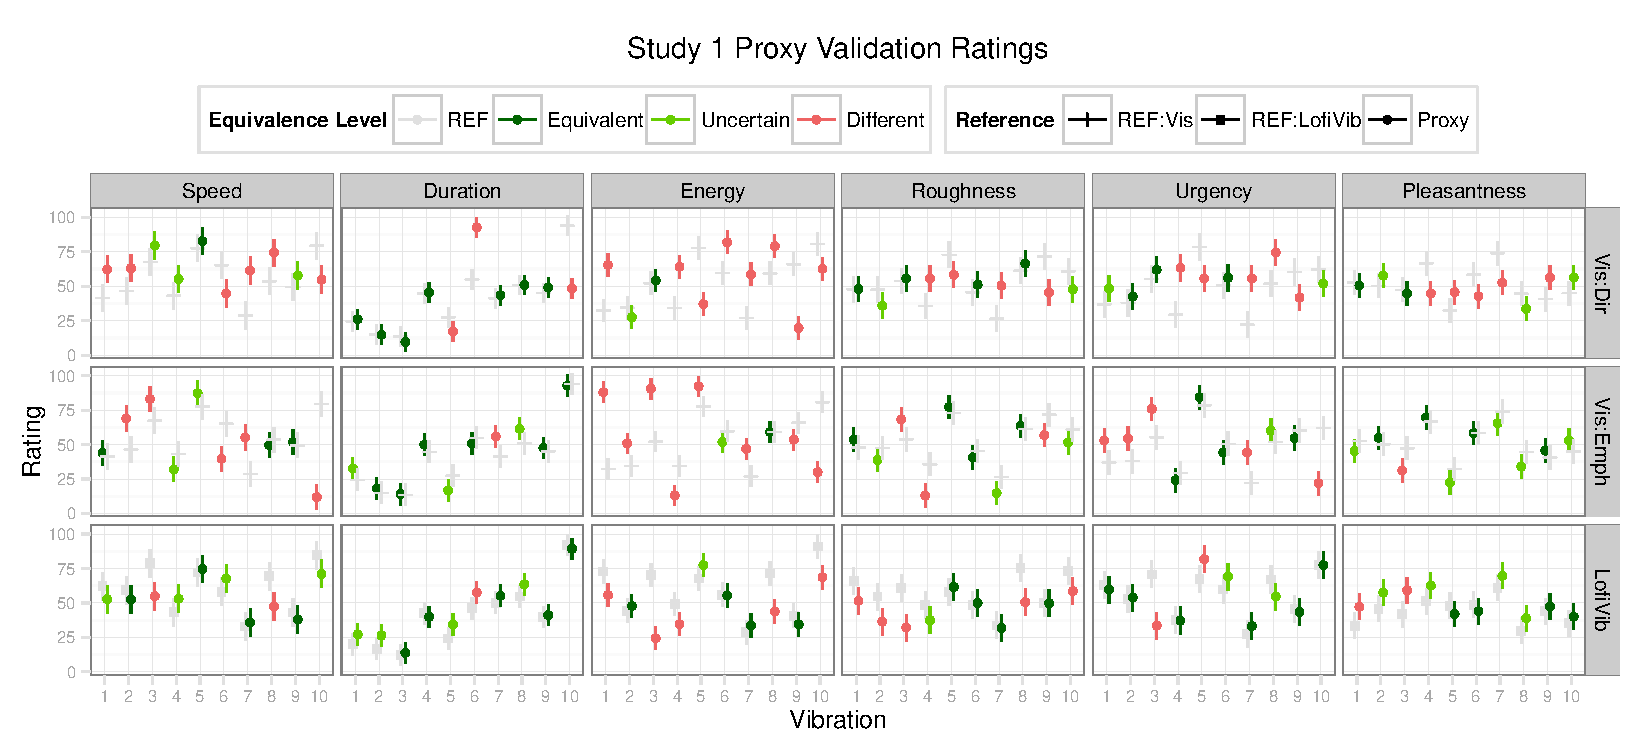
\includegraphics[width=\textwidth, height=3in]{LocalStudy-CameraReadyPlot-2015-01-08-0021}
	\caption{95\% confidence intervals and equivalence test results for Study 1 - Proxy Validation. Grey represents  \hifi~ratings. Dark green maps equivalence within our defined threshold, and red a statistical difference indicating an introduced bias; light green results are inconclusive. Within each cell, variation of \hifi~ratings means vibrations were rated differently compared to each other, suggesting they have different perceptual features and represent a varied set of source stimuli.
	}
		%\kmC{Needs explanation. SLC}
	% EXPLAIN What do dots vs bars mean. Reiterate there are three proxies (one in each row) and one 'reference', and each line/dot is a datapoint comparing one proxy method (row) for one rating type (major columns) for one of the 10 reference vibrations (minor columns). 
	% EXPLAIN how to interpret "scatter". Within a given cell, we would like to see short bars with dots close together; but its' fine, even good, for the bars to "scatter" up and down heightwise. This means users can tell them apart. The ideal result would be tight bars (black or daark green), but varying in height by vibration. If all modalities translated consistently, then the up/down pattern for vibrations will be repeated vertically across modality.  [Note: a natural but incorrect interpretation is to look for low 'scatter' within a cell, i.e. bars all close in height] 
	%SUGGEST renaming the row to indicate perceptual modality, e.g. VIS: original, VIS: Linear, VIB: Lofi.  Problem: easy to confuse "ORIGINAL" as the reference (sounds like one), instead of LOFI.  
	%SUGGEST: renaming the modalities for use throughout. get rid of ORIGINAL - it's meaning has lost relevance in this context, and its implication is confusing. Call them VIS:DIRECT, VIS:LINEAR, VIB:LOFI, VIB:REF
	% ALSO: back where defining the VIS proxies, I didn't get clear sense of why it's called LINEAR. is this the best name for it (now?) Implication is of a simplification - a linearization.  }
	
	\label{fig:results:study1}
\end{figure*}

\begin{figure}[tb]
	\centering
	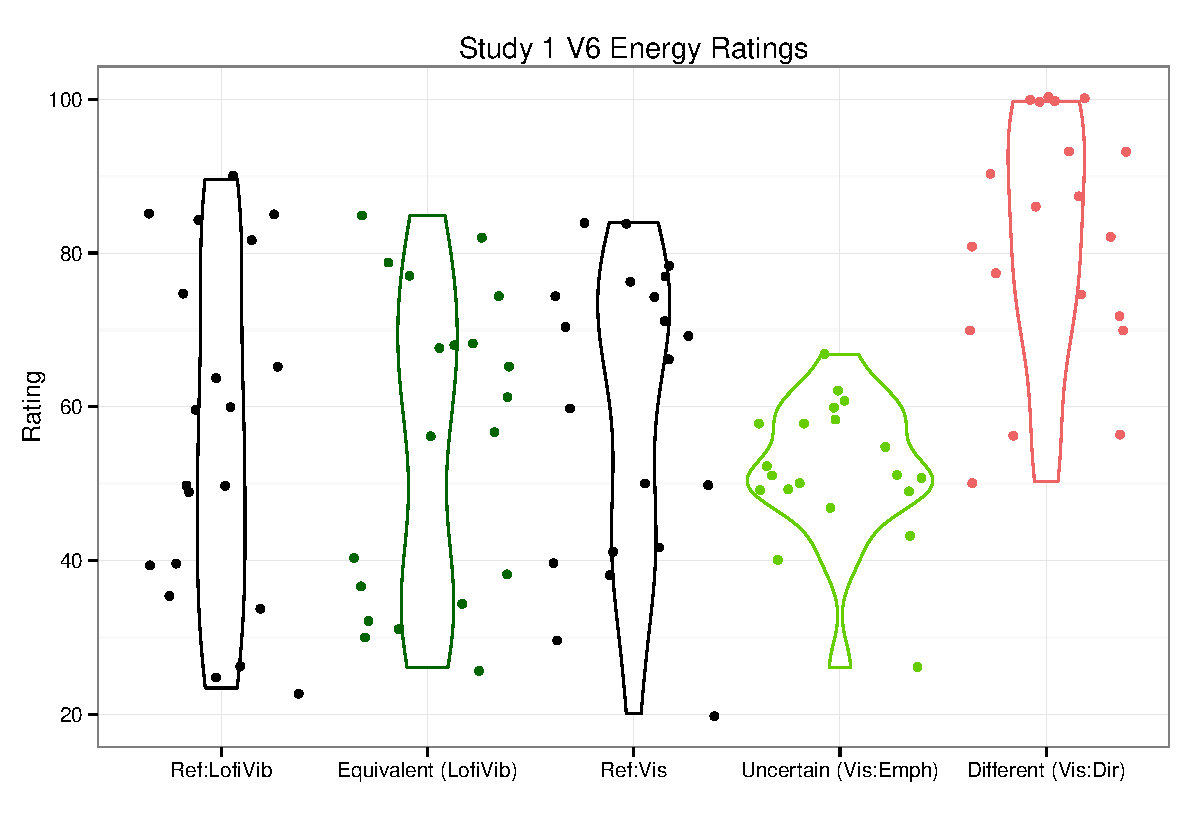
\includegraphics[width=0.6\textwidth]{Fig8-new4}
	\caption{Rating distributions from Study 1, using V6 Energy as an example. These violin plots illustrate 1) the large variance in participant ratings, and 2) how equivalence thresholds reflect the data. When equivalent, proxy ratings are visibly similar to \hifi. When uncertain, ratings follow a distribution with unclear differences. When different, there is a clear shift.}
%	\kmC{I think this is important to have, but I can't follow explanation. Also: what we can conclude from this fig for this stim, and what can you generalize to the other stim? How representative is it? minor: bigger labels}}
	\label{fig:violinplot}
\end{figure}

 \subsubsection{Duration and Pleasantness were translatable}
    Duration was comparably translatable for \lofi\ [5:1] and \linear\ [6:1]; \original\ was less consistent [7:3] (two differences very large).
    Between the three modalities, 9/10 vibrations achieved equivalence with at least one modality.
%    The remaining  two were biased (V10, the longest vibration, and V6). \kmC{explain SLC} % what does biased mean in this context? It sounds like you're saying it's okay to dismiss them because of it.
    For Duration, this is unsurprising. It is a physical property that is controllable through the Android vibration API, and both visualization methods explicitly present Duration as their $x$-axis. %. \kmC{axis? SLC} % Do you mean, they render it directly? Say how. 
    This information was apparently not lost in translation.
    
    More surprisingly, Pleasantness fared only slightly worse for \lofi\ [4:2]
    and \linear\ [4:1]; 8 / 10 vibrations had at least one modality that provided equivalence.
    %always met \hifi\ equivalence within 30 points. For \original, only two vibrations  failed this threshold. 
     Pleasantness is a higher-level affective feature than Duration.
     Although not an absolute victory, this result gives evidence that, with improvement, crowdsourcing may be a viable method of feedback for at least one affective parameter.
    
    \vspace{0.1in}
    \subsubsection{Speed and Urgency translated better with \lofi}
    	\lofi\ was  effective at representing Urgency [6:2]; \linear\ attained only  [4:5], and \original\ [3:5].
	Speed was less translatable. \lofi~did best at [4:2];
	\original~reached only [1:6], and \linear~[3:5].
	%
	However, the modalities again complemented each other.
	Of the three, 9/10 vibrations were equivalent at least once for Urgency (V8 was not).
	Speed had less coverage: 6/10 had equivalencies (V3,4,6,10 did not).
	
	\subsubsection{Roughness had mixed results; best with \linear}
    
    Roughness ratings varied heavily by vibration.
    7 vibrations had at least one equivalence (V2,4,10 did not).
    All modalities had 4 equivalencies each:
    \linear\ [4:3], \original\ [4:4], and \lofi\ [4:5]. 
    
          \subsubsection{Energy was most challenging}
          Like Roughness, 7 vibrations had at least one equivalence  between  modalities (V1,4,10 did not).
          \lofi\ [4:5] did best with Energy;
          \linear\ and \original\ struggled at [1:8]. 
          
          

%    Energy was harder in general, with 7 within a threshold of 30 for \lofi, 6 for \linear (although V7 was shockingly accurate within 10 points), and a 4 for \original.
%    Part of this could be the complexity of what ``energy" means.
%    This could also be one of the more difficult challenges when moving to proxy modalities.
%    Designing the right energy levels seems challenging for some vibrations given the current phone actuators (e.g., short pulses with high energy, very high energy signals) .
%    However, visualizations did not perform better.
%    As such, energy remains the most challenging of our 6 perceptual qualities to represent.
        %This is due the coupling of time and energy in phone actuators. i.e., the less an actuator is on, the lower the resulting energy is. Thus it is difficult to design very short strong pulses with these actuators. Also, the upper bound on the energy of phone actuators is lower than the one for C2 tactor (high-fidelity actuators). thus, designing very high-intensity vibrations is another design challenge.
    
%    In addition, designing the right energy levels seems challenging for some vibrations given the current phone actuators (e.g., short pulses with high energy, very high energy signals) while it seems more feasible with visual proxies. This suggests that triangulation of different proxies might be a good strategy. In other words, researchers can use low-fi vibrations to get user feedback on speed and urgency and collect user feedback on roughness and energy using the linear (??) proxy.
    
    \subsubsection{Emphasized visualization outperformed direct plot}
 %   \subsubsection{\linear\ outperformed \original}

	Though it depended on the vibration, \linear\ outperformed \original\ for most metrics, having the same or better equivalencies/differences for Speed, Energy, Roughness, Urgency, and Pleasantness.
	Duration was the only mixed result, as \original\ had both more equivalencies and more differences  [7:3] versus [6:1]
    %
%    \linear strictly outperformed \original for roughness, urgency, and pleasantness; for these modalities, every vibration was found equivalent at the same or higher threshold in \linear.
%    In other modalities, the results depended on the vibration, but \linear had more vibrations with higher equivalence: with speed, \linear had  6 within 30 and 3 within 20, compared to 5 and 2; with energy, \linear had 6 within 30 and 2 within 20, compared to 4 and 2 (one of which was equivalent within 10).
%    Duration has a more complex comparison: while \linear had all vibrations equivalent within a threshold of 30 (7 within threshold of 20), duration had two distinctly non-equivalence vibrations (V6 and V10), while having many very comparable ratings (three within a threshold of 20 points.
%    This suggests that \original~was more accurate at displaying some durations, while \linear~was less accurate but effective at all our vibrations.
    %
    In addition, 16/20 participants (80\%) preferred \linear\ to \original.
    Although not always clear-cut, these comparisons overall indicate that our \linear\ visualization method communicated these %perceptual
    affective qualities more effectively than the status quo.
    This supports our approach to emphasized visualization, and motivates the future pursuit of other visualizations.
    
    \subsubsection{V4,V10 difficult, V9 easy to translate}
    
    While most vibrations had at least one equivalency for 5 rating scales, V4 and V10 only had 3.
    V4 and V10 had no equivalences at all for Speed, Roughness, and Energy, making them some of the most difficult vibrations to translate.
    V4's visualization had very straight lines, perhaps downplaying its texture.
    V10 was by far the longest vibration, at 13.5s (next longest was V8 with 4.4s).
    Its length may have similarly masked textural features.
    
    V8 was not found to be equivalent for Urgency and Pleasantness.
    V8 is an extremely irregular vibration, with a varied rhythm and amplitude, and the second longest.
    This may have made it difficult to glean more intentional qualities like Urgency and Pleasantness.
    However, it was only found to be different for \original/Urgency, so we cannot conclude that significant biases exist.
    
    By contrast, V9 was the only vibration that had an equivalency for every rating scale, and in fact could be represented across all ratings with \lofi.
    V9 was a set of distinct pulses, with no dynamic ramps; it thus may have been well suited to translation to \lofi.
    
\begin{figure*}[tb]
	\centering
	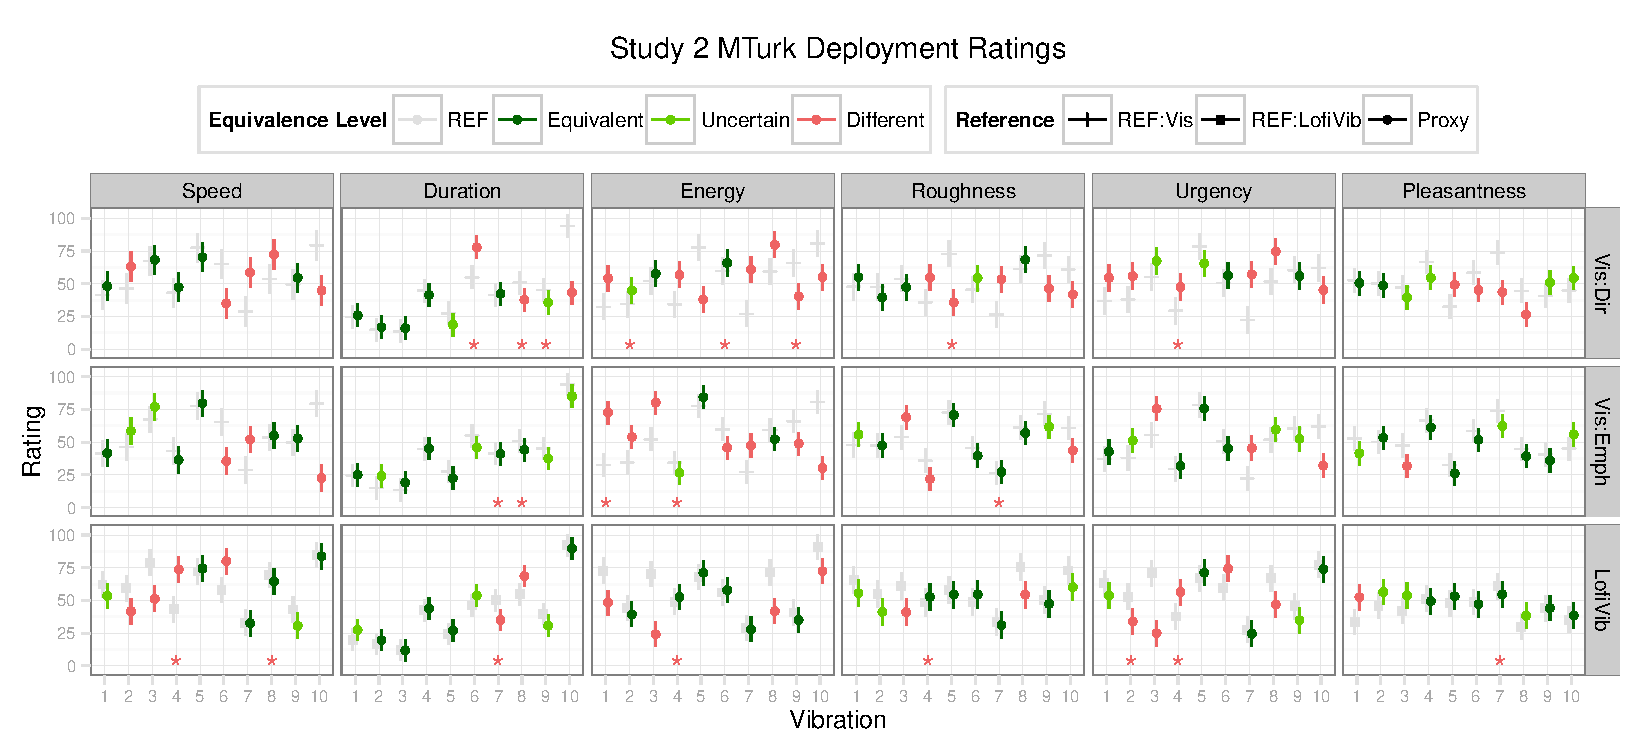
\includegraphics[width=\textwidth, height=3in]{MTurkStudy-cameraready-2015-08-0116}
	\caption{95\% Confidence Intervals and Equivalence Test Results for Study 2 - MTurk Deployment Validation. Equivalence is indicated with dark green, difference is indicated with red, and uncertainty with light green. Red star indicates statistically significant difference between remote and local proxy ratings. 
	}
	\label{fig:results:study2}
\end{figure*}

\subsubsection{Summary}
In general, these results indicate promise, but also need improvement and combination of proxy modalities.
Unsurprisingly, participant ratings varied, reducing confidence and increasing the width of confidence intervals (indeed, this is partial motivation to access larger samples). 
Even so, both differences and equivalencies were found in every rating/proxy modality pairing.
Most vibrations were equivalent with at least one modality, suggesting that we might pick an appropriate proxy modality depending on the vibration; we discuss the idea of triangulation in more detail later.
Duration and Pleasantness were fairly well represented, Urgency and Speed were captured best by \lofi, and Roughness was mixed.
Energy was particularly difficult to represent with these modalities.
%; unsurprising, as \hifi~vibrations can control frequency and amplitude simultaneously, both which have a role in energy (\ostodo CITE).
We also find that results varied depending on vibration, meaning that more analysis into what makes vibrations easier or more difficult to represent could be helpful.

Though we were able to represent several features using proxy modalities within a bounded error rate, this alone does not mean they are crowdsource-friendly.
All results from Study 1 were gathered in-lab, a more controlled environment than over MTurk.
We thus ran a second study to validate our proxy modality ratings when deployed remotely.

\section{Study 2: Deployment Validation with MTurk (G2)}
To determine whether rating of a proxy is similar when gathered locally or remotely, we deployed the same computer-run proxy modality surveys on MTurk.
We wanted to discover the challenges all through the pipeline for running a VT study on MTurk, including larger variations in phone actuators and experimental conditions (G4). 
We purposefully did not iterate on our proxy vibrations or survey, despite identifying many ways to improve them, to avoid creating a confound in comparing results of the two studies. 
% Otherwise, we might have optimized the proxies for the local study to later find out that they do not translate to a remote study 

The visualization proxies were run as a single MTurk Human Intelligence Task (HIT), counterbalanced for order; the \lofi\ survey was deployed as its own HIT.
Each HIT was estimated at 30m, for which participants received \$2.25 USD. In comparison, Study 1 participants were estimated to take 1 hour and received \$10 CAD. 
We anticipated a discrepancy in average task time due to a lack of direct supervision for the MTurk participants, and expected this to lead to less accurate participant responses, prompting the lower payrate.
On average, it took 7m for participants to complete the HIT while local study participants took 30m.

We initially accepted participants of any HIT approval rate to maximize recruitment in a short timeframe. Participants were post-screened to prevent participation in both studies. 49 participants were recruited. 
%
No post-screening was used for the visual sub-study.
%All visual proxy results were accepted. 
For the \lofi~proxy survey, we post-screened
%additional screening techniques were 
to verify device used~\cite{Mason2012conducting}. 
We asked participants (a) confirm their study completion with an Android device via a survey question (b) detected actual device via FluidSurvey's OS-check feature, and (c) rejected inconsistent samples (eg. 9 used non-Android platforms for \lofi). 
Of the included data, 20 participants participated each in the visual proxy condition (6F) and the \lofi~condition (9F).

For both studies, Study 1's data was used as a ``gold standard" that served as a baseline comparison with the more reliable local participant ratings~\cite{Amazon.comInc.2015}.
%
We compared the remote proxy results (from MTurk) to the \hifi~results gathered in Study 1, using the same analysis methods.

%40 were included in the study (9 used non-Android platforms for the \lofi HIT).


\subsection {Results}

Study 2 results appear in \autoref{fig:results:study2},
which compares remotely collected ratings with locally collected ratings for the respective reference (the same reference as for \autoref{fig:results:study1}). It can be read the same way, but adds information.
Based an analysis of a different comparison, a red star indicates a statistically significant difference between remote proxy ratings and corresponding local \textit{proxy} ratings.
This analysis revealed that ratings for the same proxy gathered remotely and locally disagreed 21 times (stars) out of 180 rating/modality/vibration combination; i.e., relatively infrequently.

Overall, we found similar results and patterns in Study 2 as for Study 1. The two figures show similar up/down rating patterns; the occasional exceptions correspond to red-starred items.
Specific results varied, possibly due to statistical noise and rating variance.
We draw similar conclusions: that proxy modalities can still be viable when deployed on MTurk, but require further development to be reliable in some cases.

% On the whole, our study 2 results mixed, but encouraging.
% For each rating/modality pair, at most three differences were detected, and more equivalencies were found than with our proxy validation.
% However, these results still indicate a large amount of noise when deploying on MTurk, with no immediate patterns about which vibrations deploy effectively.
% We discuss these results and their implications, combined with the results of Study 1, in the next section.
		
\section{Discussion}
Here we discuss high level implications from our findings and relate them to our study goals (G1-G4 in Introduction).
%	    Vibration	Duration
%V5	V10 8-24 		13.5
%V1	V7  4-20 		3.6
%V2	V1  6-5		1.5
%V3	V2  7-34		1
%V8	V9  2-40		3.1
%V4	V4  1-39		3.5
%V10 V6 1-16		3.3
%V6	V3  3-11		0.7
%V9	V5  6-27		1.1
%V7	V8  7-26		4.4

    \subsection{Proxy modalities are viable for crowdsourcing (G1,G2:feasibility)} % feasibility
   Our studies showed that proxy modalities can represent %both physical and 
   affective qualities of vibrations within reasonably chosen error bounds, depending on the vibration.
   These results largely translate to deployment on MTurk.
   Together, these two steps indicate that proxy modalities are be a viable approach to crowdsourcing VT sensations, and can reach a usable state with a bounded design iteration (as outlined in the following sections).
   This evidence also suggests that we may be able to deploy directly to MTurk for future validation.
   Our two-step validation was important as a first look at whether ratings shift dramatically; and we saw no indications of bias or overall shift between locally running proxy modalities and remotely deploying them.
   \vspace{0.35in}
    \subsection{Triangulation (G3:promising directions/proxies)}
	Most vibrations received equivalent ratings for most scales in at least one proxy modality.
	Using proxy modalities in tandem might help improve response accuracy.
	For example, V6 could be rendered with \lofi~for a pleasantness rating, then as \linear~for Urgency.
	Alternatively, we might develop an improved proxy vibration by combining modalities - a visualization with an accompanying low-fidelity vibration.
%	Taken in tandem, this might improve response accuracy.
	

    \subsection{Animate visualizations (G3:promising directions)}
    Speed and Urgency were not as effectively transmitted with our visualizations as with our vibration.
    Nor was Duration well portrayed with  \original, which had a shorter time axis than the exaggerated \linear.
    It may be more difficult for visual representations to portray time effectively: perhaps it is hard for users to distinguish Speed/Urgency, or the time axis is not at an effective granularity.
    Animations (e.g., adding a moving line to help indicate speed and urgency), might help to decouple these features.
    As with triangulation, this might also be accomplished through multimodal proxies which augment a visualization with a time-varying sense using sounds or vibration.
    Note, however, that Duration was more accurately portrayed by \linear, suggesting that direct representation of physical features \textit{can} be translated.
    
    \subsection{Sound could represent Energy (G3:promising directions)}
Our high-fidelity reference is a voice-coil actuator, also used in audio applications.
Indeed, in initial pilots we played vibration sound files through speakers. Sound is the closest to vibration in the literature, and a vibration signal's sound output is correlated with the vibration energy and sensation. 

However, in our pilots, sometimes the vibration sound did not match the sensation; was not audible (low frequency vibrations); or the C2 could only play part of the sound (i.e, the sound was louder than the sensation).

Thus, while the raw sound files are not directly translatable, a sound proxy definitely has potential. It could, for example, supplement where the \original~\ waveform failed to perform well on any metric (aside from Duration) but a more expressive visual proxy (\linear) performed better.


    \subsection{Device dependency and need for} Energy model for Vibrations (G4:challenges)
     Energy did not translate well.
     This could be a linguistic confusion, but also a failure to translate this feature.
     For the visualization proxies, it may be a matter of finding the right representation, which we continue to work on.
     
     However, with \lofi, this represents a more fundamental tradeoff due to characteristics of phone actuators, which have less control over energy output than we do with a dedicated and more powerful C2 tactor.
     The highest vibration energy available in phones is lower than for the C2;  this additional power obviously extends expressive range.
     %
     Furthermore, vibration energy and time are coupled in phone actuators: the less time the actuator is on, the lower the vibration energy.
     As a result, it is difficult to have a very short pulses with very high energy (V1,V3,V8). The C2's voice coil technology does not have this duty-cycle derived coupling.
     %
     Finally, the granularity of the energy dimension is coarser  for phone actuators.
     This results in a tradeoff for designing (for example) a ramp sensation: if you aim for accurate timing, the resulting vibration would have a lower energy (V10).
     If you match the energy, the vibration will be longer.
     
     Knowing these tradeoffs, designers and researchers can adjust their designs to obtain more accurate results on their intended metric. 
     Perhaps multiple \lofi\ translations can be developed which maintain different qualities (one optimized on timing and rhythm, the other on energy).
     In both these cases, accurate models for rendering these features will be essential.
     %[Oliver- check V9 for energy. significant in Matthew�??s analysis and has the same structure as v2,v6,v7- so makes sense to be bad on energy
      %  [Matthew based on short pulse/low energy argument, v3 should be bad in terms of energy which is not true.]
        
    %\textbf{Overall}: The biggest design challenge for android actuators seems to be having very strong, and short pulses.
        
        %Big take away: Energy could be the most important parameter!? 
        %Developing an energy model for vibrations on MTurk is critical -> provides motivation for  Oliver�??s earlier MTurk project proposal!!		
		
	\subsection{VT %Perceptual
	affective ratings are generally noisy (G4:challenges)}
   Taken as a group, participants were not highly consistent among one another when rating these %perceptual
   affective studies, whether local or remote.
  This is in line with previous work \cite{Seifi2015}, and highlights a need to further develop rating scales for affective touch.
   Larger sample sizes, perhaps gathered through crowdsourcing, may help reduce or characterize this error. Alternatively, it gives support to the need to develop mechanisms for individual customization. If there are ``types'' of users who do share preferences and interpretations, crowdsourcing can help with this as well.
   
\subsection{Response \& data quality for MTurk \lofi\ vibrations (G4:challenges)}
When deploying vibrations over MTurk, 8/29 participants (approximately 31\%) completed the survey using non-Android based OSes (Mac OS X, Windows 7,8.1, NT) despite these requirements being listed in the HIT and the survey. One participant reported not being able to feel the vibrations despite using an Android phone. 
This suggests that enforcing a remote survey to be taken on the phone is challenging, and that additional screens are needed to identify participants not on a particular platform.
Future work might investigate additional diagnostic tools to ensure that vibrations are being generated, through programmatic screening of platforms, well-worded questions and instructions, and (possibly) ways of detecting vibrations actually being played, perhaps through the microphone or accelerometer).



\subsection{Automatic translation (G4:challenges)}
Our proxy vibrations were developed by hand, to focus on the feasibility of crowdsourcing.
However, this additional effort poses a barrier for designers that might negate the benefits of using a platform of MTurk.
As this approach becomes better defined, we anticipate automatic translation heuristics for proxy vibrations using validated algorithms.
Although these might be challenging to develop for %affective
emotional features, physical properties like amplitude, frequency, or measures of energy and roughness would be a suitable first step.
Indeed, crowdsourcing itself could be used to create these algorithms, as several candidates could be developed, their proxy vibrations deployed on MTurk, and the most promising algorithms later validated in lab.



    % \subsection{Low-Fi}
    %     Duration translated well for all low-fi vibrations. 
        
       
        
        
    %     Speed did translate well except for V6, V7. [not exactly sure. for both could be the carryover impact from energy (considerably lower energy, might have felt as lower tempo too.) for V7 could be due to variations in tempo in time (too subjective??)]
        

        
        
    %     Roughness translated well except for V6,V7 (and maybe V3) but the mean differences is lower than energy. We think that roughness of the a vibration with short pulses depends on number and timing of pulses as well as the energy of each pulse. Thus, we conjecture that the smaller roughness difference for V6, V7 could be due to drastic differences in their low-fi energy. Would be interesting to find the ideal pulse duration that trade-offs the pulse energy and pulse timing (since roughness depends on both). [this argument doesn�??t cover V3, barely within range]
    %     Urgency translated well except for V6. V6 is short and rated as lower on energy, speed, and roughness, all the things that contribute to urgency. V7 is longer and have more pulses which have compensated for lack of energy and provided a higher urgency rating than V6.[again not so sure about this argument].
        
    %     Pleasantness translated well for all vibrations. In this case, V6 just barely within the range and received higher pleasantness rating than the hi-fi version. The order of pleasantness and energy ratings for those vibrations that are farther apart are the exact opposite [Interesting!!]
        
    %     Surprisingly/interestingly affective ratings of urgency and pleasantness were rated more consistently across the conditions. It could be that like people�??s criteria for affective parameters are more general. thus less impacted by small variations in physical parameters (!!) [aggressive conjecture]
        

        
        
    % \subsection{Visualization}
    % Duration translated well for all Vis L representations but not for two of Vis O representations (V5, V10). [Not sure why]
    
    % Energy did not translate well for any of the two visualization conditions. For original, the vibration height only represented the amplitude and thus energy variations due to frequency were lost (V7,V9,V1,V8,V10). This result is surprising especially for linear visualization design since we had explicitly encoded energy information on the y axis as low, medium and high. We think
    % the differences in energy for linear visualization could be due to differences in amplifier setting. We had encoded energy based on ratings from our previous user study and unfortunately we did not match the amplifier setting for this study. As a result, most vibrations were perceived to have lower energy than their visual representation. [I�??m puzzled about V4 (v1-39)]
    % [Salma- 8-24 seems to have medium energy level on VibViz interface, do you know why it�??s coded as low energy in Vis L?]
    
    % Speed did not translate well for the two visualizations either (4 and 5 error cases for VisL, and VisO respectively). The two design do not differ in their visualization of the temporal pattern of vibrations. simply reflecting the temporal pattern over time does seem to accurately reflect the perceptual speed for a vibration [why??]. In all cases that the mean speed rating for the VisL and VisO was different, VisO received higher speed rating. It could be that darker lines and filled waveshapes provide a more dense look and result in higher speed ratings. But this is only a hypothesis. 
    
    % Roughness translated well for linear visualization with one exception for V4 and only partially for VisO (except for V1, V4, V8). Interestingly for all three cases the order of roughness rating is similar to energy ratings which could speak to link between perceived energy and roughness. [cannot think of a stronger argument]
    
    % Urgency results were comparable except for three cases in VisL (), and five cases in VisO (). Many of these vibrations are among error cases for energy as well. Interestingly, in the majority of cases (9 out of 10 vibrations) the order of mean are the same for energy and urgency ratings. However, there are more drastic difference in energy ratings than urgency. 
    
    % Pleasantness ratings were comparable for all vibrations in VisL and were also comparable for VisO except for one vibration (V4). [weirdly VisL is fine for V4 although both its energy and roughness are error cases]
    
    % The challenge of providing an accurate visualization of energy is less fundamental/easier to tackle than for low-fi vibration case. We could got more promising results if we had matched the amplification levels across studies. 
    
    \subsection{Limitations}
    
    A potential confound was introduced by \linear\ having a longer time axis than \original: some of \linear's improvements could be due to seeing temporal features in higher resolution.
    This is exacerbated by V10 being notably longer than the next longest vibration, V8 (13.5s vs. 4.4s), further reducing temporal resolution vibrations other than V10.
    
    We presented ratings to participants by-vibration rather than by-rating.
    Because participants generated all ratings for a single vibration at the same time, it is possible there are correlations between the different metrics.
    We chose this arrangement because piloting suggested it was less cognitively demanding than presenting metrics separately for each vibration.
    Future work can help decide whether correlations exist between metrics, and whether these are an artifact of stimulus presentation or an underlying aspect of the touch aesthetic.
    
    \textcolor{black}{Despite MTurk's ability to recruit more participants, we used the same sample size of 40 across both studies. While our proxies seemed viable for remote deployment, there were many unknown factors in MTurk user behaviour at the time of deployment. We could not justify more effort without experiencing these factors firsthand. Thus, we decided to use a minimal sample size for the MTurk study that was statistically comparable to the local studies. In order to justify a larger remote sample size in the future, we believe it is best to iterate the rating scales and to test different sets of candidate modalities.}
    
    As discussed, we investigated two proxy modalities in this first examination but look forward to examining others (sound, text, or video) alone or in combination.
        
    %  Finally, our local study conclusions are based on a $\delta$ of 20 or 30 points on a 100-point scale
    %  While these are not a narrow band, they also represent a conservative test.
    %  The entire confidence interval for these means must lie within the range -20 to 20 or -30 to 30; many estimates that do not lie in this range also do not lie entirely out of it, and so we cannot always conclude non-equivalence for null results.
    %  Ultimately, there is uncertainty in this data; future work with larger sample sizes could help resolve whether this is due to large individual differences (observed in previous work (vibviz?)).

      
\section{Conclusion}
In this paper, we crowdsourced high-level parameter feedback on VT sensations using a new method of \emph{proxy vibrations}.
We translated our initial set of high-fidelity vibrations, suitable for wearables or other haptic interactions, into two proxy modalities: a new VT visualization method, and low-fidelity vibrations on phones.

We established the most high-risk aspects of VT proxies, namely feasibility in conveying affective properties, and consistent local and remote deployment with two user studies.
%Our two-stage evaluation (first locally testing our proxies for producing similar results as a high-fidelity reference, then deploying those same proxies in a crowdsource format and checking for similarity of results) validated the idea. It showed that proxy vibrations have the potential to gather VT feedback that is consistent with high-fidelity vibrations, even when deployed remotely over MTurk. 
Finally, we highlighted promising directions and challenges of VT proxies, to guide
%These studies provide lessons for 
future tactile crowdsourcing developments, targeted to empower VT designers with the benefits crowdsourcing brings.

% In this paper we demonstrated contributions and other contributions.
% Our contributions revealed important takeaways and highlighted a need for problem, but ultimately showed a success for goal.
% Future work will contribute further contributions on problem and related goals.
% Together, we will save the world through science.

\section{Acknowledgments}
We are grateful for participant feedback, reviewer suggestions, and extra tactors shared by Hong Tan. Research was funded by NSERC and conducted under UBC BREB H13-01646.      
%\section{Conclusion}
%In this paper, we crowdsourced high-level parameter feedback on VT sensations using a new method of \emph{proxy vibrations}.
%We translated our initial set of high-fidelity vibrations, suitable for wearables or other haptic interactions, into two proxy modalities: a new VT visualization method, and low-fidelity vibrations on phones.
%
%We established the most high-risk aspects of VT proxies, namely feasibility in conveying affective properties, and consistent local and remote deployment with two user studies.
%%Our two-stage evaluation (first locally testing our proxies for producing similar results as a high-fidelity reference, then deploying those same proxies in a crowdsource format and checking for similarity of results) validated the idea. It showed that proxy vibrations have the potential to gather VT feedback that is consistent with high-fidelity vibrations, even when deployed remotely over MTurk. 
%Finally, we highlighted promising directions and challenges of VT proxies, to guide
%%These studies provide lessons for 
%future tactile crowdsourcing developments, targeted to empower VT designers with the benefits crowdsourcing brings.
%
%% In this paper we demonstrated contributions and other contributions.
%% Our contributions revealed important takeaways and highlighted a need for problem, but ultimately showed a success for goal.
%% Future work will contribute further contributions on problem and related goals.
%% Together, we will save the world through science.



\endinput
